\documentclass[12pt]{article}

\usepackage[]{graphicx}
\usepackage[]{color}
\usepackage{alltt}

\newcommand{\mytitle}{Interpretation of black box models using tree-based surrogate models}
\newcommand{\myname}{Sofia Maria Loibl}
\newcommand{\mysupervisor}{Dr. Giuseppe Casalicchio}

\usepackage[a4paper, width = 160mm, top = 35mm, bottom = 30mm, 
bindingoffset = 0mm]{geometry}
\usepackage[utf8]{inputenc}
\usepackage{diagbox}
\usepackage{bbold}
\usepackage{makecell}
\usepackage{ragged2e}
\usepackage{xcolor}
\usepackage[nottoc]{tocbibind}
\usepackage[round, comma]{natbib}
\usepackage{fancyhdr}
\newcommand{\changefont}{%
    \fontsize{8}{11}\selectfont
}

\usepackage[onehalfspacing]{setspace}
\usepackage{amsmath}
\usepackage{hyperref}
\usepackage{enumitem}
\renewcommand{\labelenumii}{\arabic{enumii}.}
\hypersetup{
  colorlinks = true,
  linkcolor = black,
  urlcolor = black,
  citecolor = black}
\pagestyle{fancy}
\fancyhead{}
\fancyhead[R]{\changefont{\mytitle}}
\fancyfoot{}
\fancyfoot[R]{\thepage}
\setlength{\headheight}{14.5pt}
\setlength{\parindent}{0pt}
\interfootnotelinepenalty = 10000
\DeclareMathOperator*{\argmin}{arg\,min}


% ------------------------------------------------------------------------------
% MAIN -------------------------------------------------------------------------
% ------------------------------------------------------------------------------
\IfFileExists{upquote.sty}{\usepackage{upquote}}{}
\begin{document}

% FRONT PAGE -------------------------------------------------------------------
 
\begin{titlepage}
\begin{center}
    
\LARGE
Master's Thesis
    
\vspace{0.5cm}
      
\rule{\textwidth}{1.5pt}
\LARGE
\textbf{\mytitle}
\rule{\textwidth}{1.5pt}
   
\vspace{0.5cm}
      
\large
Department of Statistics \\
Ludwig-Maximilians-Universität München 

\vfill

\Large
\textbf{\myname}

\vfill

\large
Munich, March 24\textsuperscript{th}, 2023
      
\vfill


\includegraphics[width = 0.4\textwidth]{sigillum.png}

\vfill

\normalsize
Submitted in partial fulfillment of the requirements for the degree of M.Sc. in Statistik mit wirtschafts- und sozialwissenschaftlicher Ausrichtung \\
Supervised by \mysupervisor

\end{center}
\end{titlepage}

% CONTENTS ---------------------------------------------------------------------

\pagenumbering{Roman}
\newpage

\begin{abstract}

Surrogate models allow complex but powerful black box machine learning models to be interpreted retrospectively. In this work, the following requirement is placed on a surrogate model: It should divide the feature space in subregions where interpretable models that only include main effects can approximate the black box model. In this way, both good interpretability and high performance should be achieved. For the generation of such models, four different model-based tree algorithms  are compared: SLIM, GUIDE, MOB and CTree. Selection bias, performance, interpretability and stability of the different methods are investigated. In the presence of subgroup-specific main effects, SLIM and GUIDE convince with their results regarding interpretability and performance.

\end{abstract}

\newpage
\tableofcontents

%%%% if you would want to include material overview
%%%% use one of the following in addition
% \newpage
% \listoffigures
% \newpage
% \listoftables
\newpage

% CHAPTERS ---------------------------------------------------------------------

\pagenumbering{arabic}
    
\section{Introduction}
\label{intro}
Various machine learning algorithms achieve outstanding predictive performance nowadays. However, most of them are complex black box models that, unlike traditional statistical methods such as linear regression, are not intrinsically interpretable \citep{Hu.2020}.
Especially in highly regulated industries such as insurance, this is a problem \citep{Henckaerts.2022}.
In order to maintain the good performance of complex black box models but still achieve a certain degree of interpretability, there exist different methods with which models can be interpreted post-hoc. 


One option are so called surrogate models. The idea is to approximate the predictions of black box models by intrinsically interpretable models \citep{Molnar.2019}.
But in order for a surrogate model's explanations to be trusted, it must itself perform well in approximating the black box predictions.
There are basically two approaches for generating surrogate models: global surrogate models, which cover the entire feature space and can be interpreted globally, but often do not perform that well, or local surrogate models, which only explain individual observations.  The focus of this work is on a mixture of the two approaches, which are called subregional surrogate models here. 
The idea is to find subregions in the feature space in which intrinsically interpretable models can be fitted.


Model-based tree (MBT) algorithms are a promising class to generate such subregional models. 
The concept of MBTs is based on classical regression trees like CART \citep{Breiman.1984} but a MBT contains models instead of constant values in the subregions (called nodes or leaf nodes).
It is hence a combination of decision rules and models. If intrinsically interpretable models are chosen for the models, a principally interpretable MBT is derived. The degree of interpretability and performance, though, depends on the complexity of the decision rules (i.e. depth of the tree or number of leaf nodes) and of the models.
In order to enable a good interpretability of the models in the leaf nodes, this thesis sets the constraint that only main effect models are fitted in the nodes. 
In the ideal case, interactions should then be handled by  splits, so that the models in the leaf nodes are free from interaction effects.
To ensure that the splits are actually due to interactions and not to nonlinearities, it is necessary that potentially nonlinear main effects are modelled appropriately.
Although in some cases linear modelling of the main effects is sufficient, it should also be possible to fit more complex models, such as (penalized) polynomial models or generalised additive models (GAM).
The goal is thus an additive decomposition of a black box function by combining decision rules and additive main effect models.  In other words
subregions in the feature space should be found, so that the global black box model can be replaced by subregional main effect models.


In my research, I found four different algorithms that can generate MBTs. 
The most recent approach Surrogate Locally-Interpretable Models (SLIM) by \cite{Hu.2020} allows a high flexibility in the choice of model classes in the leaf nodes. SLIM uses an exhaustive search to find the best split point through all possible splitting variables. 
In this thesis SLIM is contrasted with three common algorithms for creating MBTs: Model-based recursive Partitioning (MOB) \citep{Zeileis.2008}, Conditional Inference Trees (CTree) \citep{Hothorn.2006} and Regression tress with unbiased variable selection and interaction detection (GUIDE) \citep{Loh.2002}. These algorithms differ from SLIM mainly in that the search for the best split point is a two-step process. First, the best split variable is selected by a hypothesis test, which differs between the three algorithms. Then, in a second step, the best split point for this variable is searched. Since certain prerequisites must be fulfilled for the hypothesis tests, the choice of model classes for these algorithms is limited to some extent. 

The comparison of the four algorithms is made with the condition that main effect only models are fitted in the nodes and all features are included in the search for the splitting variable. First, it is examined how the algorithms differ in terms of selection bias. Afterwards, they are compared with regard to their performance, interpretability and stability, as tree algorithms often suffer from poor stability \citep{Fokkema.2020}. In the subsequent application to data sets from the area of life insurance, their suitability as surrogate models is examined.

The main results of this thesis are that SLIM and GUIDE are particularly successful in terms of performance, interpretability and stability when subgroup specific maineffects are present in the data. Smooth interactions are partially better modelled by MOB and CTree. In general for data with smooth interactions all four algorithms produce models with a large number of subregions when high performance is required. The MBTs are then difficult to interpret and less suitable as surrogate models. Furthermore, when applied to the insurance data, it is noticeable that the deeper the MBTs are, the more similar the performance of the different algorithms becomes.

The thesis is structured as follows:
In chapter \ref{related}, an overview of surrogate models is given and MBTs are placed in this setting. Thereafter, the four MBT algorithms are described in chapter \ref{background}. Chapter \ref{selection} examines the extent to which the algorithms suffer from selection bias. In chapter \ref{simulation}, different simulation scenarios are used to examine how the algorithms differ in terms of performance, interpretability and stability. In addition, the interpretability and performance of the SLIM algorithm are examined when the complexity of the leaf node models is varied. Finally, in chapter \ref{usecase} the algorithms are used as surrogate models for the modelling of insurance data and different SLIM models are used for interpretation. 


\newpage

\section{Related work}
\label{related}
\subsection{Global surrogate models}

\subsection{Local surrogate model}

\subsection{Sub-regional surrogate models}

\newpage

\section{Model-based trees}
\label{background}
\subsection{Model and Notation}
Following \citep{Zeileis.2008} and \citep{Seibold.2016}, let $\mathcal{M}((y, \mathbf{x}), \theta)$ be a parametric model, that describes the target $y \in \mathcal{Y}$ as a function of a feature matrix $\mathbf{x} = (\mathbf{x_1}, ... \mathbf{x_p})^T \in \mathcal{X}$  and a vector of parameters $\mathbf{\theta} \in \Theta$. When the model is used as a surrogate model, $y$ is the prediction of the black box model that should be explained.  If it must be explicitly stated that the response is the prediction of a black-box model, the notation $y^{bb}$ is used. Given $n$ observations $(y, \mathbf{x}) = (y^{(1)}, \mathbf{x}^{(1)}),..., (y^{(n)}, \mathbf{x}^{(n)})$ the model can be fitted by minimizing some objective function $\Psi((y, \mathbf{x}), \theta)$ yielding the parameter estimate $\hat{\theta}$
\begin{align}
    \hat{\mathbf{\theta}} = \argmin_{\theta \in \Theta} \sum_{i=1}^{n}\Psi(y^{(i)}, \mathbf{x}^{(i)}, \theta).
\end{align}

In this thesis $\mathcal{M}((y, \mathbf{x}), \theta)$ is restricted to additive main-effect regression models.. However, if the data includes interactions, a single global model is not sufficient to fit all $n$ observations well.  To deal with interactions, the idea is to partition the feature space $\mathcal{X}$ into subregions $\{\mathcal{B}_b\}_{b = 1,...,B}$ and search for locally well fitting main-effect models in these regions. The global objective function thus expands to
\begin{align}
    \sum_{b=1}^B\sum_{i \in I_b}\Psi(y^{(i)}, \mathbf{x}^{(i)}, \theta_b)
\end{align}
and has to be minimized over all partitions $\{\mathcal{B}_b\}$ (with corresponding indexes $I_b, b = 1,...,B$) and local optimal parameter $\theta_b$ for each partition. As \citep{Zeileis.2008} points out, it is very difficult to find the optimal partition, because the number of possible partitions quickly becomes too large for an exhaustive search.





\subsection{Model-based Trees}
In this chapter, four algorithms are described that aim to find a partition that is close to the optimal one and the associated estimators for $\theta_b$ through binary recursive partitioning. All approachs use a greedy forward search to optimize the objective function $\Psi$ locally in each step \citep{Zeileis.2008}.  
The resulting global models are called Model-based Trees (MBT).



A recursive partitioning algorithm for MBTs can generally be divided into the following steps:
\begin{enumerate}
    \item Start with the partition (node) $I_0 = 1,...,n$
    \item Fit the model to all observations in the current node $\{y^{(i)}, \mathbf{x}^{(i)}\}, i \in I_b$ by estimating $\hat{\theta}_b$ via minimization of the objective function $\Psi$
    \item Find the local optimal splitpoint for this node 
    \item If no stop criterion is met (e.g. depth of the tree, improvement of the objective through split, significance of parameter instability) split the node in two child nodes and repeat the steps 2-4.
\end{enumerate}


The algorithms SLIM, MOB, CTree and GUIDE considered in this work can be divided into two groups. SLIM falls into the group of biased recursive partitioning algorithms, which also includes classical methods like AID \citep{Morgan.1963} and CART \citep{Breiman.1984}. These algorithms use an exhaustive search to select the optimal split point in step 3. This can lead to the phenomenon that, even if the strength of all feature effects (or in our case interaction effects) are the same, fetaures with many possible split points are more often chosen as split variables than fetaures with few possible split points. This phenomenon is called selection bias and is explained in more detail in \ref{selection} and examined for the algorithms considered here.
MOB, CTree and GUIDE are assigned to unbiased recursive partitioning. Instead of comparing the objective for all possible split points and variables, step 3 of the recursive partitioning algorithm is split into 2 steps:

\begin{enumerate}
    \item Select the variable that has the highest association with the response as splitting (partitioning) variable. The tests to determine the most significant association differ between the methods.
    \item Search for the best split point only within this variable (e.g. by exhaustive search or again by hypothesis testing)
\end{enumerate}

\citep{Schlosser.2019}



\subsubsection{SLIM}
SLIM by \citep{Hu.2020} is explicitly designed to create surrogate MBTs that contain main effect models in the leafnodes and are split by interactions. 

After fitting the model to all observations in step 2 the  objective function is calculated, e.g. the sum of squared errors (SSE).
In step 3 SLIM performs an exhaustive search to find the optimal splitpoint.  
The optimization problem in each recursion step includes the optimization of the objective of the left node and the right node and is given by \begin{align} \label{align:mob_opitimization}
    \min_{j \in 1,..., p} \left( \min_{s \in \mathcal{S}_j} \left(\min_{\theta_{l} \in \Theta}\sum_{i \in I_{l}(s)}\Psi(y^{(i)}, \mathbf{x}^{(i)}, \theta_{l})  +  \min_{\theta_{r} \in \Theta}\sum_{i \in I_{r}(s)}\Psi(y^{(i)}, \mathbf{x}^{(i)}, \theta_{r}) \right) \right),
\end{align}
where ${S}_j$ is the set of all possible split points $s$ (or split sets) regarding variable $\mathbf{x}_j$. For numeric variables, this set consists either of all unique values of $\mathbf{x}_j$ or, in order to reduce the calculation effort, of sample quantiles (e.g. 100 quantiles). For a specific split point $s$, the left node $I_{l}$ is defined as the set of indices $i \in 1,...,n$ for which $x_j^{(i)} \leq s$ holds and the right node $I_{r}$ is its complement. For categorical variables, all possibilities of dividing the levels of $\mathbf{x}_j$ into two disjoint sets are considered as potential split sets $S_j$. $I_l$ is  the set of all indices for which $x_j^{(i)} \in s$ applies and and $I_{r}$ is its complement.

The variable $\mathbf{x}_j$ and split point $s$ which minimize  (\ref{align:mob_opitimization}) are selected as splitting variable and split point, if this leads to a large enough improvement of the objective function.

Since the computational effort for estimating all possible child models becomes very large as the number of possible partitioning variables increases, \citep{Hu.2020} have developed an efficient algorithm for estimating them for the case of linear regression, linear regression with bspline transformed features and ridge regression. A detailed description of this algorithm can be found in \citep{Hu.2020}.

To avoid overfitting and to obtain a small interpretable tree, the use of pruning is necessary. \citet{Hu.2020} use the approach of backpruning, i.e. a deep tree is first fitted and then leaves that do not fulfil certain criteria are pruned back. 
In order to keep the computational effort as low as possible, prepruning is used in this thesis. Specifically, this means that a split is only performed if the improvement of the objective through the split is at least $impr \in [0,1]$ times the improvement of the objective in the parent node. In addition, it is possible to set a value for $R^2$ (defined in chapter \ref{simulation}) above which splitting in a node will not continue.




\subsubsection{MOB}
MOB generally distinguishes between regressor variables $\mathbf{x}$, which are only used to fit the models in the nodes, and pure partitioning variables $\mathbf{z}$. In \citep{Zeileis.2008}, however, an overlapping of roles is explicitly not excluded. 
In this thesis, the roles should not be defined in advance, but all features should be able to enter the MBT both as main-effect and in the splits as interactions.
In this way, the application of MOB in this thesis differs from other application examples as in \citet{Seibold.2016} or \citet{Thomas.2018}. 



After an initial model has been fitted in step 2, MOB examines whether the corresponding parameter estimates $\hat{\theta}_b$ are stable. If there is some overall instability, the variable whose parameter estimate has the most significant instability is chosen as splitting variable.

To investigate this, the so called score $\psi$ function is considered, which is defined as the
gradient of the objective function regarding the parameter vector $\theta_b$ - provided that it exists:

\begin{align}
    \psi \left( \left(y, \mathbf{x} \right), \theta_b \right) = \frac{\partial \Psi\left( \left(y, \mathbf{x} \right), \theta_b \right)}{\partial \theta_b}.
\end{align}

\citep{Zeileis.2008}


In contrast to the definition in \citet{Zeileis.2008}, $\textbf{z} = \textbf{x}$ was set in (\ref{align:W_j}) as no distinction is made between regressor and partitioning variables.
If the scores - ordered by the potential split variable - do not fluctuate randomly around zero, this indicates that there is parameter instability which could potentially be captured by splitting the data using this variable as partitioning variable \citep{Schlosser.2019}.
To test the null hypothesis of parameter stability with the so called M-fluctuation test, MOB captures systematic deviations from zero through the empirical fluctuation process

\begin{align}\label{align:W_j}
    W_{j}(t) = \hat{J}^{-1/2}n^{-1/2}\sum_{i = 1}^{\lfloor nt \rfloor} \hat{\psi}_{\sigma(x_{j}^{(i)})} \hspace{0.5cm} (0 \leq t \leq 1), 
\end{align}

where $\hat{\psi}_{\sigma(x_{j}^{(i)})}$ are the scores ordered by $\mathbf{x}_{j}$ and $\hat{J}$ is an estimate of the covariance matrix $cov(\psi(Y, \hat{\theta}))$. \citep{Zeileis.2008}




According to \citet{Zeileis.2008} and \citet{Zeileis.2007}, under the null hypothesis of parameter stability the empirical fluctuation process $W_j(t)$ converges to a Brownian Bridge $W_0$. By applying a scalar test function to the empirical fluctuation process and the Brownian Bridge, a test statistic and the theoretical limiting distribution can be derived. An overview of possible scalar functions that can be used for this purpose can be found in \citep{Zeileis.2008} and in more detail in \citep{Zeileis.2007}.
The variable for which the M-fluctuation test detects the most significant parameter instability is used as splitting variable. 

The choice of the optimal split point with respect to this variable is then made by means of an exhaustive search, analogous to SLIM.

As a prepruning criterion, MOB uses the Bonferroni-adjusted p-value of the M-flucutation test. That means a split is only performed if the instability is significant at a given significance level $alpha$.


A limitation of MOB is that only objective functions can be selected for which the gradient regarding $\theta_b$  exists. This means, for example, that it is not possible to fit LASSO models in the nodes.




\subsubsection{CTree}
CTree was originally developed as a non-parametric regression tree (i.e. constant fits in the leaf) but can also be used for MBTs.
CTree follows a very similar approach to MOB and also tries to detect parameter instability by analysing the dependency between potential splitting variables and a transformation $h()$ of the response $y$.
A common transformation used in MBTs is the score function, i.e. $h(y) = \psi$, but other transformation of the response variable that can detect instabilities in the estimates could also be used. A simple alternative would be to use the residuals. According to \citep{Schlosser.2019}, however, the use of the scores - if they exist - is preferable, since instabilities can be better detected with them.

To test the independence between the scores and the potential partition variables, CTree uses a linear association test.

To measure the association between the scores $y$ and a potential splitting variable $\textbf{x}_{j}, j = 1,...,p$ a linear statistics of the form 
\begin{align}
    T_{j}(y,\textbf{x}) = vec\left(\sum_{i=1}^n \textbf{x}_j^{(i)}\hat{\psi}^{(i)T}\right) \in \mathbf{R}^{p_{j} q}
\end{align}
is used which is derived from the more general definition in \citep{Hothorn.2006}.

To standardize the teststatistic $T_{j}$, the conditional expectation and covariance of $T_{j}$ under the null hypothesis of independence between $y$ and $\textbf{x}_j$ given all permutations of $\{y,\textbf{x}\}$ are calculated.
Different transformations can be used to to map the multivariate test statistic $T_{j}$ to a standardized univariate test statistic. The default setting in the R package $\mathtt{partykit}$  \citep{Hothorn.2015b} is a quadratic transformation for numerical features. According to  \citep{Hothorn.2006} the transformed teststatistic follows an asymptotic $\chi^2$ distribution under the nullhypothesis.
As in MOB, the splitting variable, for which the p-value of the test is the smallest is selected as splitting variable. A Bonferroni-adjusted p-value is again used as prepruning criterion.



Unlike the other methods, the split point is not selected by an exhaustive search, but with the help of a linear test statistic. The discrepancy between two subsets is measured with a two-sample linear test statistic for each possible binary split. The split that maximises the discrepancy is chosen as the split point. \citep{Hothorn.2006}

\citet{Schlosser.2019} state that the linear test used in CTree has higher power in detecting smooth relationships between the scores and the splitting variables compared to the M-fluctuation test in MOB. MOB, on the other hand, has a higher ability in detecting abrupt changes.


\subsubsection{GUIDE}
GUIDE \citep{Loh.2002} uses residual-based categorical association tests to detect instabilities. For this purpose, $\chi^2$- independence tests between the dichotomized residuals of the fitted model and the categorized covariates are performed and the p-values of these so-called curvature tests are calculated. In addition to the curvature tests, GUIDE explicitly searches for interactions.  Again, $\chi^2$- independence tests are performed. Instead of categorizing only one variable, a new categorical variable is created by combining covariates for the interaction test. If the smallest p-value comes from a curvature test, the corresponding covariate is chosen as the partitioning variable. If the smallest p-value is from an interaction test, the categorical variable involved, if any, is preferably chosen as the splitting variable. If both potential variables are categorical, the variable for which the p-value of the curvature test is smaller is chosen. In the case of two numerical variables, the choice is made by evaluating the potential child models after splitting with respect to both variables.
Subsequently, a bootstrap selection bias correction is performed.
In the original GUIDE algorithm developed by \citep{Loh.2002}, numerical variables can be used both as regressor variables and as splitting variables. Categorical variables, on the other hand, can only take on the role of splitting variables. This is justified by the fact that a disproportionately large number of degrees of freedom are consumed in the parameter estimation of categorical variables.
In the following simulations, both a GUIDE implementation in which categorical variables can only serve as splitting variables and a variant in which categorical variables can also take on both roles are considered. 

One advantage of GUIDE is that the score function does not have to exist. This makes the choice of objective very flexible and allows, for example, to fit LASSO regression models  in the nodes.




\subsection{Software implementation}

No implementation of SLIM was found, which is why an implementation in R  \citep{RCoreTeam.2022} was carried out as part of this work. The code from the package $\mathtt{customtrees}$ from \citet{Casalicchio.2020} and from \citet{Herbinger.2022} was used as basis. The source code for the SLIM implementation and the applications in this thesis can be found at \url{https://github.com/slds-lmu/msc_2022_loibl_thesis}. 

The software implementation of GUIDE falls in the category "Algorithms with a closed-source, free-of-charge implementation" \citep{Loh.2014}. The binary executable is available under \url{https://pages.stat.wisc.edu/~loh/guide.html}.  Unfortunately, the source code is not accessible and the method cannot be easily adapted to other objectives, although this would be theoretically possible. For this reason, I have incorporated the residual based $\chi^2$- independence tests for finding the best split variable as an option of the SLIM implementation in R  in this work. Bootstrap bias correction was also adopted. To the best of my knowledge, I followed the original paper \citep{Loh.2002}. However, the results differ somewhat from the results in the paper, as can be seen in the appendix in figure \ref{}. 
Whenever GUIDE is discussed in the following, it refers to my implementation. 

MOB and CTree are implemented in the R package $\mathtt{partykit}$ \citep{Hothorn.2015} in the functions $\mathtt{mob()}$ \citep{Zeileis.2008} and $\mathtt{ctree()}$ \citep{Hothorn.2006}




\subsection{Comparison}

In Table \ref{tab:mbt_comparison} a comparison of the different MBT algorithms is given. SLIM and GUIDE are particularly interesting because of their flexibility in choosing different loss functions. In the case of SLIM, one open question is whether the exhaustive search, in contrast to the two-step methods, leads to a selection bias. This will be examined in the following chapter \ref{selection}.
\begin{table}[ht]
\centering
\begin{tabular}{lllll}
  \hline
 & Split point selection & Test & Flexibility & Implementation  \\ 
  \hline
    SLIM & exhaustive search & - & high & - \\ 
    MOB & two-step & score-based fluctuation & low & R package \\ 
    CTree & two-step & score-based Permutation & low & R package\\ 
    GUIDE & two-step & residual-based $\chi^2$  & high & binary executable\\ 
   \hline
\end{tabular}
\label{tab:mbt_comparison}
\end{table}
%\citep{Schlosser.2019}



\newpage

\section{Selection bias and splitting strategies}
\label{selection}
\subsection{Definition and motivation}

According to \citep{Hothorn.2006} an algorithm for recursive partitioning is called unbiased when, under the conditions of the null hypothesis of independence between a response $y$ and feature $\textbf{x}_{1},...\textbf{x}_{p}$ the probability of selecting feature $\textbf{x}_{j}$ is $1/p$ for all $j = 1,...,p$ regardless of the measurement scales or number of missing values. 

This definition may be surprising at first, since if there is no dependency between the target and the features, one would not want to perform a split anyway and would try to prevent this through appropriate pruning procedures.
However, the idea behind this is that if, in the case of independence, a feature with, for example, a large number of possible split points is selected more frequently as a splitting variable than a feature with a smaller number of split points, the former could also be incorrectly selected more frequently as a splitting variable if there is a dependency on the response for the second feature.
\citep{Loh.2014}

In the discussion on the Paper Fifty Years of Classification and Regression Trees of \citep{Loh.2014}, Carolin Strobl's statement on selection bias is therefore very clear:
\vspace{0.5cm}


{\par\centering \textit{"One should think that the results shown here [...] are so clear that any statistically educated person should never
want to use a biased recursive partitioning algorithm again."}\par}
\vspace{0.5cm}

So if SLIM is the only biased algorithm, it would have to be discarded immediately according to this statement. However, this will be investigated in detail in the following.



\subsection{Simulation independence scenarios}
In order to empirically investigate whether the four algorithms presented actually correspond to the respective groups (biased and unbiased) using the definition of \citet{Hothorn.2006}, two different simulation were carried out.

In the first scenario only numerical features are used, whereas in the second scenario numerical features and additionally one binary and two categorical features are considered.

\paragraph{Independence numeric\\}
The data in the first scenario is defined as follows:
\begin{itemize}
    \item $\textbf{x}_{1}, \textbf{x}_{2} \sim U(0,1)$
    \item $\textbf{x}_3$ uniformly distributed on the set $\{0, 0.1,..., 0.9, 1\}$
    \item $\textbf{x}_4$ uniformly distributed on the set $\{0, 0.01,..., 0.99, 1\}$
    \item $y \sim N(0,1)$
    \item sample size $n = 1000$
    \item 1000 simulation runs
\end{itemize}

The resulting frequencies are shown in Figure \ref{fig:selection_bias_independence_numeric} and are consistent with the expectations. SLIM clearly prefers to select features with a higher number of split points and therefore is biased. The other three methods seem to  select all four features about the same number of times.

\begin{figure}[!htb]
    \centering
    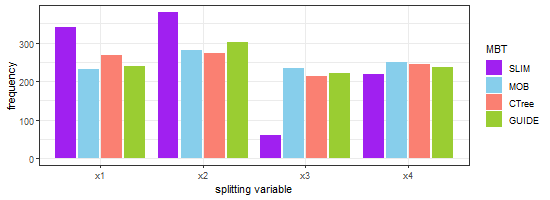
\includegraphics[width=10cm]{Figures/simulations/chapter_4_selection_bias/selection_bias_general/independence_numerical.png}
    \caption{Simulated frequencies of selected splitting features for scenario independence numeric}   \label{fig:selection_bias_independence_numeric}
\end{figure}



\paragraph{Selection bias independence mixed \newline} 
In the second scenario, the data is simulated as follows:
\begin{itemize}
    \item $\textbf{x}_{1}, \textbf{x}_{2} \sim U(0,1)$ 
    \item $\textbf{x}_3$ uniformly distributed on the set $\{0, 0.1,..., 0.9, 1\}$ 
    \item $\textbf{x}_4  \sim Bern(0.5)$ 
    \item $\textbf{x}_5$ uniformly distributed on 5 factor levels (15 possible splits) 
    \item $\textbf{x}_6$ uniformly distributed on 8 factor levels (128 possible splits) %stirling number of second kind    
    \item $y \sim N(0,1)$
    \item sample size $n = 1000$
    \item 1000 simulation runs
\end{itemize}

The addition of categorical features in this scenario results in a different picture for the frequencies, as shown in Figure \ref{fig:selection_bias_independence_mixed}. Although the numerical variables are chosen with approximately equal frequency in the so-called "unbiased" methods, there are large deviations in the binary and categorical variables especially for MOB and CTree, which calls the designation "unbiased" into question. 
A possible explanation for this selection bias could be that due to the large number of parameters that have to be estimated for the categorical features in the modelling step, random dependencies to the target variable are already caught well in the model  and therefore these variables are used less frequently as splitting variables.


In \citep{Hothorn.2006} the unbiasedness of CTree is empirically investigated for cases, in which a strict separation between regressor variables and partitioning variables is kept. Therefore, the result shown here should not principally question the label, but it does not seem appropriate when there is an overlap or, as in our case, even congruence between the two roles.


\begin{figure}[!htb]
    \centering
    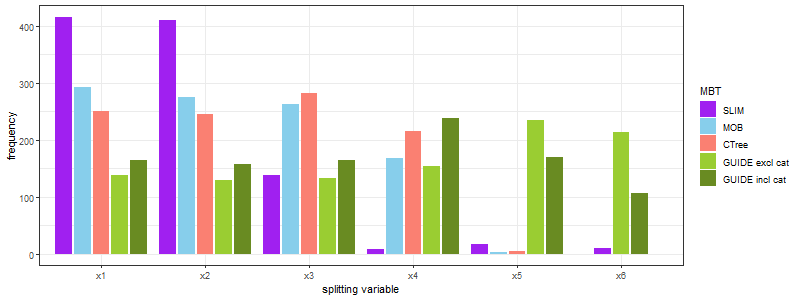
\includegraphics[width=14cm]{Figures/simulations/chapter_4_selection_bias/selection_bias_general/independence_mixed.png}
    \caption{Simulated frequencies of selected splitting features for scenario independence mixed}
    \label{fig:selection_bias_independence_mixed}
\end{figure}

For GUIDE two different variants were evaluated in this scenario. "GUIDE excl cat" corresponds to the original version, in which categorical features are only used as splitting and not as regressor variables. In "GUIDE incl cat", on the other hand, the categorical features are also used as regressors. The fact that the frequencies of the categorical variables are smaller in "GUIDE incl. cat" could be explained analogously to the selection bias of MOB and CTree.

The binary feature $\textbf{x}_4$ is almost never chosen as a splitting variable with SLIM, in contrast to the other variables. However, this can be attributed to the selection bias in numerical features with different numbers of split points, as the binary variable can be seen as numerical variable with only one possible split point. What is more interesting is that the numerical variable $\textbf{x}_2$ with 10 possible split points is chosen by SLIM much more frequently as splitting variable than the variable $\textbf{x}_6$ with 128 possible splits, so that the bias cannot be determined by the number of possible splits alone.

The difference between the categorical ($\textbf{x}_5$ and $\textbf{x}_6$) and the numerical variables can probably be explained in a similar way as with the other methods, but in reverse. With SLIM, the potential split is executed first and then models in the child nodes are fitted.  If a numerical feature is used as partitioning variable, the parameters for all factor levels are estimated in both child models, whereby random dependencies with $y$ can be modelled very accurately. If, on the other hand, splitting is done according to a categorical variable, only a subset of the factor levels can be used for modelling in both child nodes.






As a possible correction approach for the selection bias in SLIM, I investigated how the number of quantiles considered as potential split points affects the selection bias and the performance of SLIM. The simulation setup and results are shown in the appendix \ref{app:selection_bias_correction}. In summary, although selection bias can be reduced for numerical variables in the case of an independent target variable, this correction can lead to unpredictable biases if interactions are actually present. For this reason, the approach is not recommended. 
For all simulations in this chapter, each unique value was seen as a potential split point for SLIM.






\subsection{Simulation interaction scenarios} \label{selection_bias_interactions}
While so far only the frequencies with which different feature types are selected in the case of independence were shown, it is empirically investigated in the following which feature types the different MBT algorithms tend to select when interactions are actually present.
Four different scenarios are examined for this. These are, in a sense, pair comparisons of different feature types. In all scenarios, the data generating process consists of two pairs of interactions, whereby the interactions have the same strength. Each pair consists of a numerical variable that enters linearly into the interaction and another variable that splits the linear effect into two subgroups.
In all four scenarios the numerical variables which define the linear effect are 
 $\textbf{x}_{2}, \textbf{x}_{4} \sim U(0,1)$ .

The features $\textbf{x}_{1}$ and $\textbf{x}_{3}$ are responsible for the subgroups. They are uniformly distributed on sets, which are given in Table \ref{tab:selection_bias_interaction}, as well as the data generating processes.

\begin{table}[!htb]
    \centering
    \begin{tabular}{llll}
        \hline
        scenario & $\textbf{x}_1$ & $\textbf{x}_3$ & $f(\textbf{x})$\\
        \hline
        numerical vs numerical & $[0,1]$ &  $\{0, 0.1,..., 0.9, 1\}$ & $\mathbb{1}_{(\textbf{x}_1 \leq  mean(\textbf{x}_1))}\textbf{x}_2  +  \mathbb{1}_{(\textbf{x}_3 \leq  mean(\textbf{x}_3))}\textbf{x}_4 $ \\
        binary vs categorical & $\{0,1\}$ &  $\{a,b,c,d,e,f\}$ & $\mathbb{1}_{(\textbf{x}_1 = 0)}\textbf{x}_2  +  \mathbb{1}_{(\textbf{x}_3 \in \{a,b,c\})}\textbf{x}_4 $ \\
        numerical vs binary & $[0,1]$ & $\{0,1\}$ & $\mathbb{1}_{(\textbf{x}_1 \leq  mean(\textbf{x}_1))}\textbf{x}_2  +  \mathbb{1}_{(\textbf{x}_3 = 0)}\textbf{x}_4$ \\
        numerical vs categorical & $[0,1]$ & $\{a,b,c,d,e,f\}$ & $\mathbb{1}_{(\textbf{x}_1 \leq  mean(\textbf{x}_1))}\textbf{x}_2  +  \mathbb{1}_{(\textbf{x}_3 \in \{a,b,c\})}\textbf{x}_4$ \\
        \hline
    \end{tabular}
    \caption{Simulation scenarios selection bias interaction}
    \label{tab:selection_bias_interaction}
\end{table}





All experiments are repeated 1000 times. The error terms are set to $\epsilon \sim N(0, 0.1 \cdot sd(f(\textbf{x}))$ and the data generating processes are $y = f(\textbf{x}) + \epsilon$.



First of all, there is the question of how selection bias should be defined in these scenarios. Transferring the definition from the independence case, one possibility would be to require that the frequency of being selected as a split variable for all features is 1/4.  However, this does not take into account that splits according to $\textbf{x}_1$  and $\textbf{x}_3$ , i.e. according to the split features that define the subgroups, produce a considerable greater improvement in performance than splits according to the smooth features $\textbf{x}_2$  and $\textbf{x}_4$. If $\textbf{x}_1$  and $\textbf{x}_3$  are chosen preferentially, one should not regard this as selection bias but as a good splitting strategy to get the smallest and best performing trees possible. What could be expected from an unbiased procedure, however, is that both interaction pairs are chosen equally often for the first split.



\begin{figure}[!htb]
    \centering   
    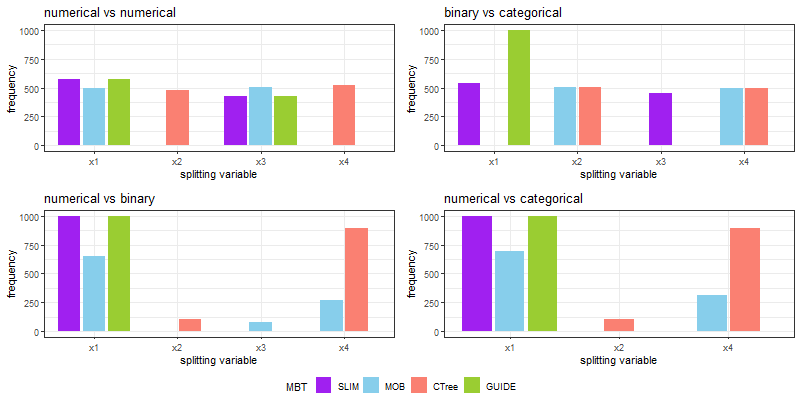
\includegraphics[width = 16cm]{Figures/simulations/chapter_4_selection_bias/selection_bias_general/interactions.png}
    \caption{Simulated frequencies of selected splitting features for the four interaction scenarios}
    \label{fig:selection_bias_interactions}
\end{figure}

Figure \ref{fig:selection_bias_interactions} shows the frequencies of the first selected split variable in each scenario for each MBT. It can be seen that in none of the scenarios and for none of the MBTs the results seem to be equally distributed among all four features. 
As a general rule, it is noticeable that SLIM and GUIDE always prefer the subgroup-defining variables ($\textbf{x}_1$  and $\textbf{x}_3$) for splitting, while CTree always prefers the smooth variables. For MOB, the behaviour varies depending on the feature type.

In Scenario "numerical vs numerical", the distribution for MOB and CTree is at least evenly distributed between the two interactions pairs. One could therefore speak of unbiasedness here. However, while CTree only uses the linear features $\textbf{x}_2$ and $\textbf{x}_4$ as the first split variable, MOB splits according to the subgroup-defining features, which is preferable in practice.
In GUIDE and SLIM, only the features $\textbf{x}_1$ and $\textbf{x}_3$ are selected, but there seems to be a preference for the variable $\textbf{x}_1$, which has a larger number of potential split points.


In the scenario "binary vs categorical", the distribution between the two interaction pairs seems to be roughly equal for SLIM, MOB and CTree. In contrast to the first scenario, MOB does not split according to the subgroup-defining variables but with regard to the linear features.
In GUIDE, only the binary variable is selected, so there is a clear preference for the binary variable over the categorical variable.

In the remaining scenarios, a strong selection bias is evident in all MBTs. SLIM, for example, gives considerable preference to numerical subgroup-defining variables over binary and categorical variables.





Obviously, these scenarios do not represent a complete overview of possible interactions. However, since MBTs can show their strengths especially in the presence of subgroup-specific maineffects (i.e. good interpretability through small trees but good performance at the same time), only such scenarios are compared here. These simulation results should sensitise to the fact that in certain cases variables could only be selected as splitting variables because they have certain properties and not because their share in an interaction is actually the largest, even with the so-called unbiased methods.

Finally it should be noted that even if selection bias is present in the independence case, this does not necessarily lead to the wrong variable being selected for splitting. In particular, this can often be prevented by pruning. However, as far as could be observed here, selection bias is very difficult to control or predict and should therefore always be considered when using these algorithms.





%\textbf{Test for selection bias:} $\chi^2$ goodness of fit test\\
%H0: the probabilities of the population are all equal (or are equal to an assumed probability distribution p)






\newpage

\section{Comparison of performance, interpretability and stability}
\label{simulation}
What should be checked by the simulations?
\begin{itemize}
    \item SLIM Accuracy (Train/Test)
    \item SLIM Fidelity (Train/Test)
    \item Blackbox Accuracy (Train/Test)
    \item Interpretability (e.g. number of leaf nodes)
    \item Stability (e.g. number of occurence of unique structures of a tree (barplot) \citep{Zhou.2018}, adjusted Rand index (ARI) \citep{Schlosser.24.06.2019}
\end{itemize}


What scenarios are we interested in?
\begin{enumerate}
    \item basic scenario linear: relatively simple linear model with few predictors and interactions (can possibly be omitted)
    \item basic scenario nonlinear: simple nonlinear model with few predictors and interactions 
    \item complex scenario nonlinear:  complex nonlinear model with many predictors and interactions 
    \item sparse scenario: basic scenario + multiple noise variables (Lasso Regression)
    \item Multicollinearity: basic scenario with correlated predictors (Lasso or Ridge Regression)
    \item skewed scenario: basic scenario + skewed distribution of the predictors
    \item outlier scenario: basic scenario + need for a robust regression
    \item selection bias scenario: Simulate probability of variable selection when the respone is independent of all variables \citep{Hothorn.2006}
\end{enumerate}

\newpage
\clearpage

\section{Insurance use case}
\label{usecase}
In the following, SLIM is used in various configurations as a surrogate for modelling the benefit present values of two fictitious insurance tariffs from the TRAIL.X (TRustworthy Artificial Intelligence in Life Insurance) research project \citep{msginsurit.16.03.2023}. The results are interpreted and the fidelity is compared with the MBT algorithms GUIDE, MOB and CTree.

\subsection{Data set K2204}
The data set K2204 contains data for a (fictitious) endowment insurance tariff. With this tariff, a single benefit is paid both in the event of survival and death of the policyholder. The data set includes the features sex (1 = male, 0 = female), age and duration and the two targets benefit present value (BPV) and premium present value (PPV). The targets were modelled using two different black box models.  
In the following, only the BPV is considered. The results for the PBV are very similar (interpreted the other way round) and can be found in the appendix.
Since the data set with 5994 observations is rather small, all observations were used for training. For this data set therefore only training performance of the surrogate models is considered.
A special characteristic of K2204 is a correlation between the features age and duration, as can be seen in Figure \ref{fig:ins_corr_age_duration}. When interpreting a MBT for this data set, it must therefore be taken into account that a split with regard to one of the features can have an influence on the value range of the other feature.

\begin{figure}[!htb]
    \centering    
    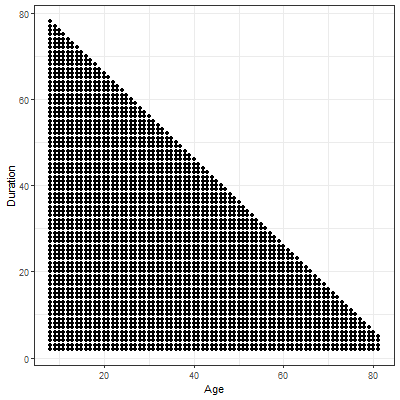
\includegraphics[width=5cm]{Figures/insurance_use_case/k2204_BPV/corr_age_duration.png}
    \caption{Features age and duration in the K2204 data set}
    \label{fig:ins_corr_age_duration}
\end{figure}


\subsubsection{Shallow MBTs with linear models}
In a first step, SLIM was fitted as surrogate to the black box predictions of BPV (BPV\_pred) with linear regression models in the nodes. The maximum depth was set to 3 and an improvement in the objective ($impr$) of at least $0.1$ of the previous improvement was set as prepruning parameter.
 The resulting tree is shown in Figure \ref{fig:ins_slim_lm_tree}.

 \begin{figure}[!htb]
     \centering     
     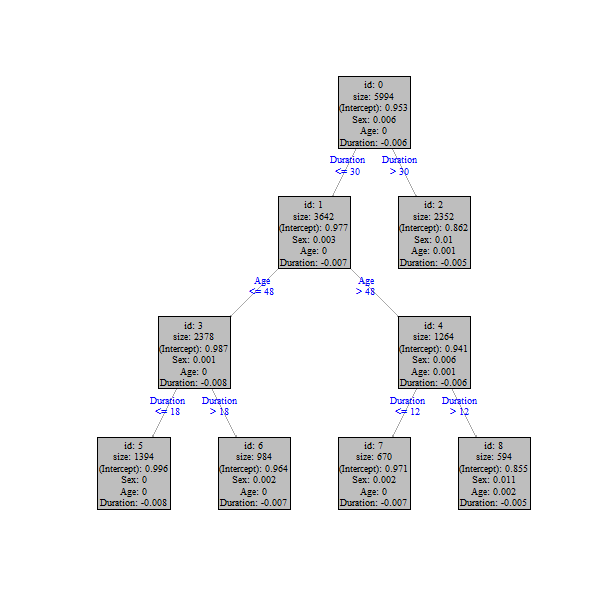
\includegraphics[width = 14cm]{Figures/insurance_use_case/k2204_BPV/slim_lm_tree.png}
     \caption{SLIM tree for K2204 with linear models}
     \label{fig:ins_slim_lm_tree}
 \end{figure}

Basic observations across all subregions are:
\begin{itemize}
    \item Gender male has a positive effect on BPV\_pred
    \item age has a positive effect on BPV\_pred
    \item duration has a negative effect on BPV\_pred
\end{itemize}

The strength of the effects, however, differs in the different subregions found by SLIM.
The five leafnodes can be roughly divided into two regions with similar effects:
\begin{itemize}
    \item Region 1 (Nodes 2,8): High duration ($30$) or high age ($>48$) and medium duration (between $13$ and $30$)
    \item Region 2 (Nodes 5,6,7): Low - medium duration with low age or high age with low duration ($\leq 12$)
\end{itemize}

In Region 1 sex male and age seem to have a higher positive effect on  BPV\_pred than in region 2. The negative effect of duration, on the other hand, is smaller in region 1. This indicates a non-linearity of duration.

If SLIM is fitted as a standalone model instead of a surrogate model in the same configuration, the differences in the split points are very small. This indicates that the black box model captures the underlying relationships very well. The corresponding tree is shown in the appendix in Figure \ref{fig:app_ins_slim_lm_standalone_tree}.

In the following, the fidelity of the different MBT with algorithms with linear models is compared. For this purpose, all four algorithms were fitted with a maximum depth of 3. For SLIM and GUIDE, $impr$ is set to $0.05$ and for MOB and CTree $alpha$ is set to $0.05$. Furthermore, a minimum nodesize of 200 observations is required.
The MBTs are compared with a baseline model, which is a linear regression model on the entire feature space. In addition to the $R^2$ and the MSE, the mean absolute error (MAE) and the maximum absolute error (max AE) are included as measures of fidelity. The max AE is particularly important here, as it is strictly regulated in order not to discriminate against any individual. 
The results are listed in table \ref{tab:ins_k2204_lm_surrogates_perf}. It shows that all MBTs achieve considerable improvement over the baseline model.

\begin{table}[!htb]

\caption{Fidelity of K2204 linear baseline model and linear MBTs}
\centering \scriptsize
\begin{tabular}[t]{l|r|r|r|r|r}
\hline
  & $R^2$ & MSE & MAE & max AE & n leaves\\
\hline
linear baseline model & 0.985101 & 0.000201 & 0.011393 & 0.064709 & 1\\
\hline
SLIM & 0.999233 & 0.000010 & 0.002272 & 0.020526 & 8\\
GUIDE & 0.999276 & 0.000010 & 0.002142 & 0.020526 & 8\\
MOB & 0.998527 & 0.000020 & 0.003149 & 0.024504 & 8\\
CTree & 0.995091 & 0.000066 & 0.005740 & 0.042931 & 8\\
\hline
\end{tabular}
\label{tab:ins_k2204_lm_surrogates_perf}
\end{table}

GUIDE achieves the best performance slightly ahead of SLIM. CTree obtains the worst performance.
Since all algorithms generate MBTs with the same number of leafnodes, the difference in performance must be explained by different split features or points.
Table \ref{tab:ins_k2204_lm_surrogates_share} lists the share of observations that were split with respect to the different features.

\begin{table}[!htb]

\caption{Share of observations split by the different features K2204 linear MBTs}
\centering \scriptsize
\begin{tabular}[t]{l|r|r|r}
\hline
& age & duration & sex\\
\hline
SLIM & 0.28 & 0.67 & 0.05\\
GUIDE & 0.28 & 0.72 & 0.00\\
MOB & 0.10 & 0.77 & 0.13\\
CTree & 0.00 & 0.96 & 0.04\\
\hline
\end{tabular}
\label{tab:ins_k2204_lm_surrogates_share}
\end{table}

It is noticeable that SLIM and GUIDE split by age more often than the other two algorithms.

\subsubsection{MBTs with B-spline models}

In order to better capture non-linearities and thus reduce the risk of splitting with respect to non-linearities instead of interactions, all MBT algorithms are fitted with B-spline transformed feature age and duration as surrogate models. 
Two different maximal depths are used, 3 for interpretable shallow trees and 6 for deep trees with higher fidelity. The settings for $alpha$, $impr$ and minimum nodesize remain the same as for the MBTs with linear models.  Again, a baseline model is fitted, in this case a regression model with the feature sex and B-spline transformed features age and duration on the entire feature space. 

Figure \ref{fig:ins_k2204_fit} plots the prediction of the baseline B-spline model and the two B-spline SLIM surrogates against BPV\_pred to visualise performance improvement. This shows a considerable improvement from the baseline model to the shallow tree. For the deep tree, the observations seem to be even somewhat closer to the identity line. 

\begin{figure}[!htb]
    \centering    
    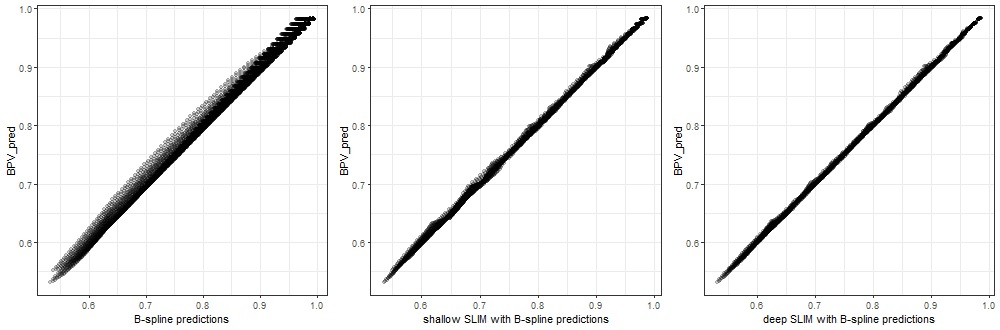
\includegraphics[width = 14cm]{Figures/insurance_use_case/k2204_BPV/fit.png}
    \caption{B-spline surrogate predictions vs. BPV\_pred for K2204}
    \label{fig:ins_k2204_fit}
\end{figure}

The fidelity results for all B-spline surrogates are listed in table \ref{tab:ins_k2204_bsplines_surrogates_perf} .

\begin{table}

\caption{Fidelity of K2204 B-spline baseline model and  B-spline MBTs}
\centering \scriptsize
\begin{tabular}[t]{l|r|r|r|r|r}
\hline
  & $R^2$ & MSE & MAE & max AE & n leaves\\
\hline
B-spline baseline model & 0.9943311 & 7.63e-05 & 0.0067811 & 0.0378568 & 1\\
\hline
SLIM shallow & 0.9994176 & 7.80e-06 & 0.0018244 & 0.0167730 & 8\\
GUIDE shallow & 0.9993900 & 8.20e-06 & 0.0019011 & 0.0165545 & 8\\
MOB shallow & 0.9992115 & 1.06e-05 & 0.0022236 & 0.0182034 & 8\\
CTree shallow & 0.9990918 & 1.22e-05 & 0.0024194 & 0.0183906 & 8\\
\hline
SLIM deep & 0.9997514 & 3.30e-06 & 0.0010766 & 0.0126778 & 21\\
GUIDE deep & 0.9997301 & 3.60e-06 & 0.0011730 & 0.0116453 & 20\\
MOB deep & 0.9996858 & 4.20e-06 & 0.0013448 & 0.0119785 & 21\\
CTree deep & 0.9997091 & 3.90e-06 & 0.0012936 & 0.0123686 & 20\\
\hline
\end{tabular}
\label{tab:ins_k2204_bsplines_surrogates_perf}
\end{table}


The improvement of the shallow MBTs over the baseline model is large, but not as substantial as in the trees with linear models without B-spline transformations. This is probably due to the fact that the splits in the MBTs with linear models also handled non-linearities that could not be adjusted in the linear baseline model. In the baseline model with B-spline transformations, on the other hand, the non-linearities are already taken into account and the splits then actually capture primarily the interactions, which is what is desired. 
The deeper splitting improves the performance of all MBTs considerably. The MAE of the deep trees, for example, is only 52\%-61\% of the MAE of the shallow trees. CTree achieves the greatest improvement and obtains better fidelity in the deep trees than MOB (except for max AE). The better performance of all MBTs, however, comes at the cost of interpretability. Additionally, there is an increased risk of overfitting.


Table \ref{tab:ins_k2204_bsplines_surrogates_share}  shows the proportions of observations that were split according to the different features. 


\begin{table}[!htb]
\caption{Share of observations split by the different features K2204 B-spline MBTs}
\centering \scriptsize
\begin{tabular}[t]{l|r|r|r}
\hline
  & age & duration & sex\\
\hline
SLIM shallow & 0.38 & 0.62 & 0.00\\
GUIDE shallow & 0.30 & 0.70 & 0.00\\
MOB shallow & 0.08 & 0.84 & 0.08\\
CTree shallow & 0.23 & 0.71 & 0.07\\
\hline
SLIM deep & 0.35 & 0.60 & 0.04\\
GUIDE deep & 0.20 & 0.78 & 0.02\\
MOB deep & 0.08 & 0.76 & 0.16\\
CTree deep & 0.20 & 0.67 & 0.13\\
\hline
\end{tabular}
\label{tab:ins_k2204_bsplines_surrogates_share}
\end{table}

For SLIM, GUIDE and MOB the share results of the shallow trees are similar to the MBTs with linear models. Shallow CTree, on the other hand, selects age in $23\%$ of split observations as splitting variable, whereas it was not used at all for splitting in CTree with linear models. It performs the worst in terms of fidelity in this case as well, but not as considerable as in the previous setting.
With the deep trees, the values for share and also the fidelity values of the different MBTs move closer together.



For the interpretation, the shallow SLIM B-spline tree is analysed in more detail.

\begin{figure}[!htb]
    \centering   
    \includegraphics[width = 16cm]{Figures/insurance_use_case/k2204_BPV/slim_bsplines_small_tree.png}
         \caption{SLIM tree for K2204 with B-spline models}
     \label{fig:ins_slim_bsplines_tree}
\end{figure}

In order to investigate the effects of the splits on the feature effects more closely, the splits with regard to duration and age are analysed separately.
The nodes 1,5,13 and 14 together comprise the entire feature space, whereby the sub-regions are determined by splits with regard to the feature duration.
Figure \ref{fig:ins_k2204_effects_duration} shows the input-output relation (feature effects) of the features estimated in the B-spline models in the different nodes. Note that the curves are centred.

\begin{figure}[!htb]
    \centering
    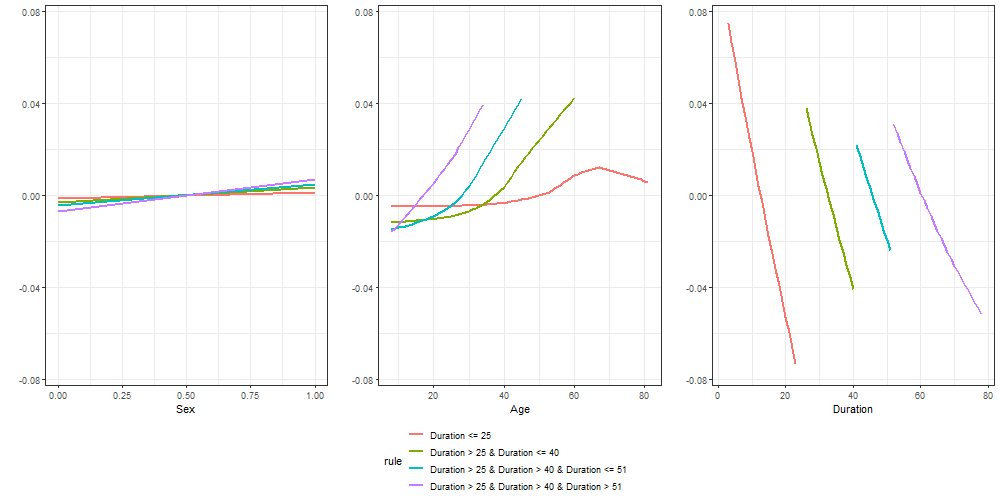
\includegraphics[width = 16cm]{Figures/insurance_use_case/k2204_BPV/effects_duration.png}
    \caption{Input-output relation of features in nodes split by duration for SLIM tree with B-splines and depth 3}
    \label{fig:ins_k2204_effects_duration}
\end{figure}

As with SLIM with linear models, it can be seen that the positive effect of sex male seems to increase with increasing duration. The same applies to age. The seemingly negative effect of age at low duration and high age is probably due to extrapolation, as there are only
few observations in this area, which is shown in Figure \ref{fig:ins_k2204_hist_age}.

\begin{figure}[!htb]
    \centering
    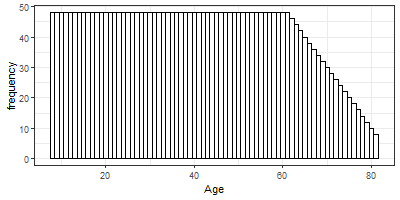
\includegraphics[width = 12cm]{Figures/insurance_use_case/k2204_BPV/hist_age.png}
    \caption{Frequency of observations with respect to feature age}
    \label{fig:ins_k2204_hist_age}
\end{figure}

With the feature duration, it can be seen that the negative effect seems to decrease with increasing duration, which is again just a non-linearity.

To investigate the effect of splits with respect to feature age, on the one hand nodes 4,7 and 8 are compared, which cover the featurespace for duration $\leq 25$, and on the other hand nodes 11 and 12, which cover the featurespace for $25 > $duration $<= 40$. In the Figures \ref{fig:ins_k2204_effects_age_low_duration} and \ref{fig:ins_k2204_effects_age_medium_duration} the corresponding input-output relations of the features are shown.

\begin{figure}[!htb]
    \centering    
    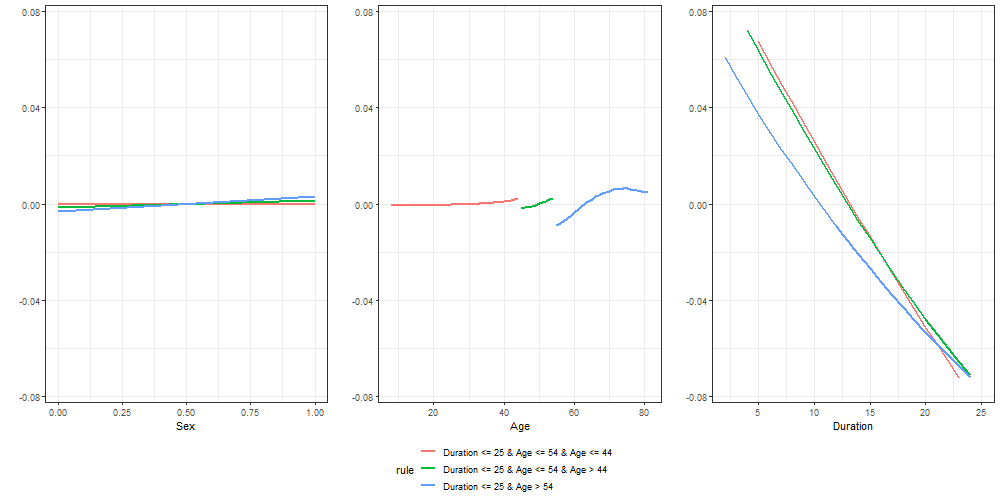
\includegraphics[width = 16cm]{Figures/insurance_use_case/k2204_BPV/effects_age_low_duration.png}
    \caption{Input-output relation of features in nodes with duration $\leq 25$ split by age for SLIM tree with B-splines and depth 3}
    \label{fig:ins_k2204_effects_age_low_duration}
\end{figure}

\begin{figure}[!htb]
    \centering    
    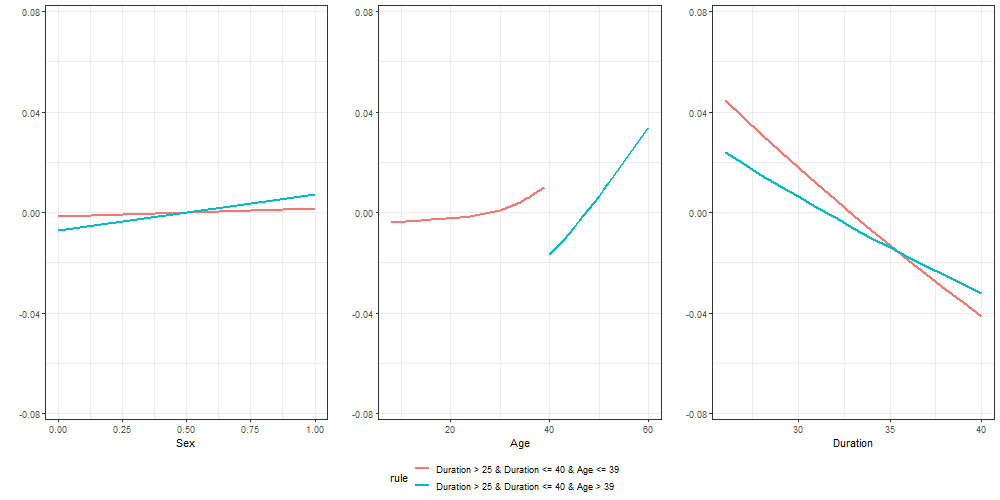
\includegraphics[width = 16cm]{Figures/insurance_use_case/k2204_BPV/effects_age_medium_duration.png}
    \caption{Input-output relation of features in nodes with $25 > $duration $<= 40$ split by age for SLIM tree with B-splines and depth 3}
    \label{fig:ins_k2204_effects_age_medium_duration}
\end{figure}

Again, the interpretation is consistent with the results from SLIM with linear models. The positive effect of sex and age is increased by increasing age, while the negative effect of duration is reduced. The slightly negative effect of age at high age and low duration should again be viewed with caution and is probably due to the poor data situation in this area.


Finally, a deep SLIM tree with B-spline models is used as a standalone model for BPV and its accuracy is compared to the accuracy of the black box model. The result is shown in Table \ref{tab:ins_k2204_standalone_slim}.
The accuracy of SLIM is worse than that of the black box model for all evaluation measures. However, the difference is most apparent for the max AE. While the max AE is explicitly minimised in the black box model, the MSE is minimised with SLIM. In general, a different loss function would also be possible with SLIM. In this case, either the max AE could be minimised only in the split selection, or also in the modelling in the nodes. When optimising the max AE in the split selection, it must be noted that the algorithm is principally designed for additive loss functions. In order to compare the joint performance of the child models with that of the parent model, the maximum should probably be used instead. 
However, it is questionable whether the data would be split according to interactions in this case, especially if the models were nevertheless fitted using least squared regression.

\begin{table}[!htb]

\caption{Accuracy of standalone B-spline SLIM MBTs and of the black box model K2204}
\centering \scriptsize
\begin{tabular}[t]{l|r|r|r|r}
\hline
  & $R^2$ & MSE & MAE & max AE \\
\hline
SLIM & 0.9997757 & 3.1e-06 & 0.0010172 & 0.0118951\\
Blackbox model & 0.9998316 & 2.3e-06 & 0.0009441 & 0.0047668\\
\hline
\end{tabular}
\label{tab:ins_k2204_standalone_slim}
\end{table}








\subsection{Data set R1\_08}

The data set R1\_08 contains the data of an annuity insurance tariff. Instead of a single benefit in the endowment case, a lifelong annuity is paid out.
R1\_08 includes, in addition to sex, age and duration, the features birth\_year, payment\_period, in\_year\_payments\_exkasso (categorical with 4 levels), guarantee\_period and increment\_factor.
The value range of the features age and duration is limited to a range in which no correlation exists ($25 \leq$ age $\leq 35$ and $30 \leq$ duration $\leq 40$).
Here, as well, the BPV or BPV\_pred is analysed as target variable. Here, as well, the BPV and BPV\_pred predicted by a black box model are analysed as target variables.
For the application of the MBTs, subsets of the training and test datasets including BPV and BPV\_pred are drawn, each with 100000 observations.

In order to model non-linearities in the nodes, MBTs with B-spline models are used. As with K2204, trees with two different depths are evaluated, shallow trees with a maximum depth of 3 and deep trees with a maximum depth of 7. $impr$ and $alpha$ are set to 0.05 and a minimum nodesize of 500 observations is required.

For the interpretation of the splits and models, the shallow SLIM tree is examined in more detail. Its structure is shown in Figure \ref{fig:ins_k108_slim_bsplines_small_tree}.

\begin{figure}[!htb]
    \centering
    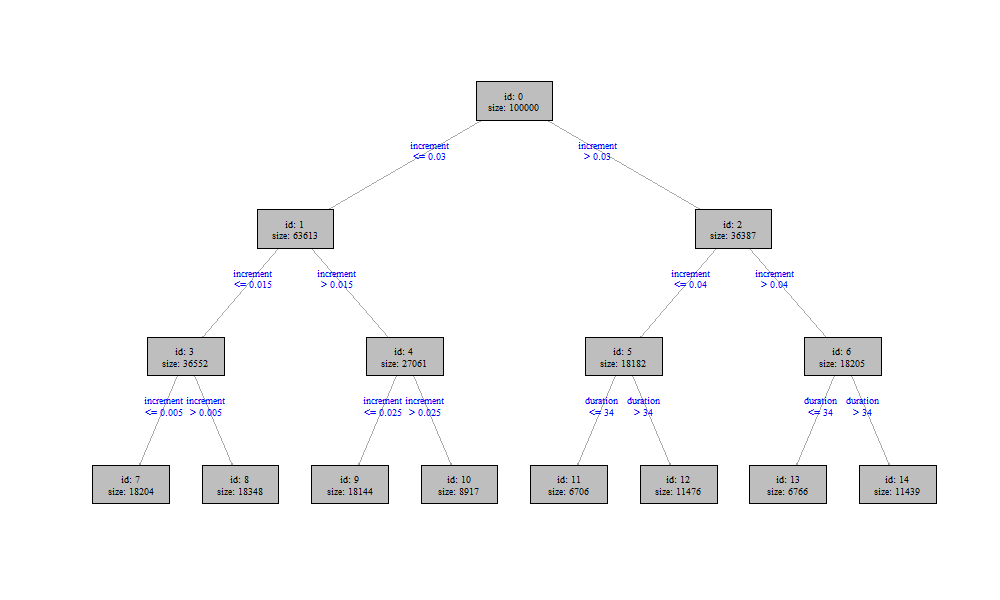
\includegraphics[width = 16cm]{Figures/insurance_use_case/k1_08_BPV/slim_bsplines_small_tree.png}
    \caption{Shallow SLIM tree for K1\_08 with B-spline models}
    \label{fig:ins_k108_slim_bsplines_small_tree}
\end{figure}

If the tree is fitted on the test data instead of the training data, exactly the same splits result. The same applies if the tree is used as a standalone model for BPV instead of a surrogate model. This indicates that the black box model replicates the true data and relationships well.
It is noticeable that the featurespace in the first splits is only divided with regard to increment\_factor. The effects of these splits on the other features are shown in Figure \ref{fig:ins_k108_effects_increment}.

\begin{figure}[!htb]
    \centering    
    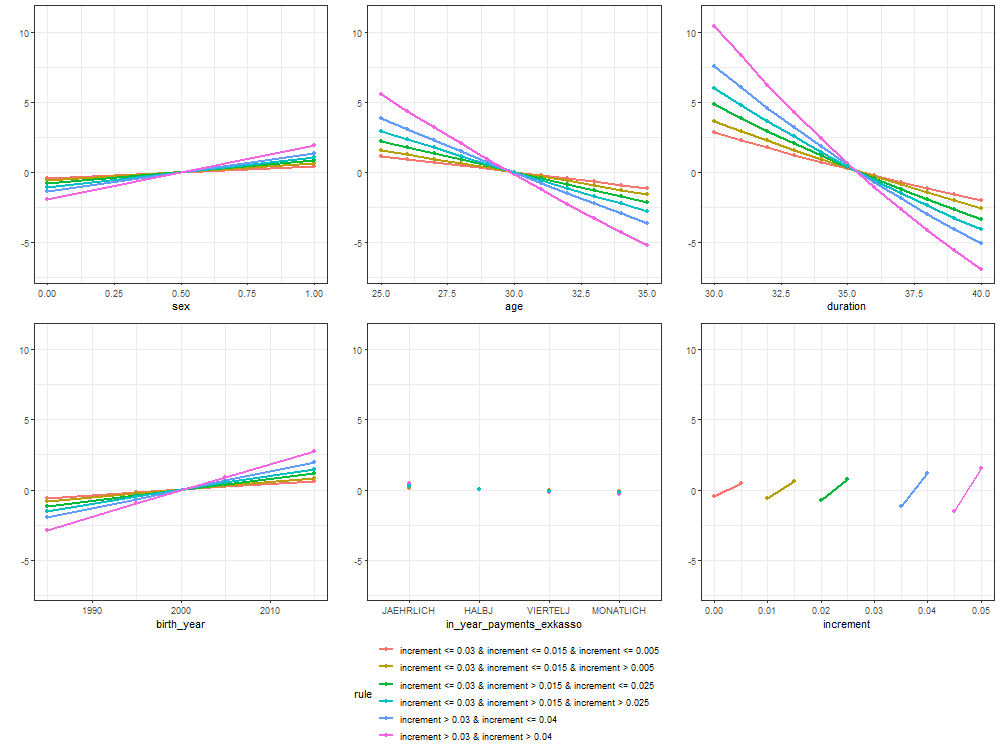
\includegraphics[width=16cm]{Figures/insurance_use_case/k1_08_BPV/effects_increment_factor.png}
    \caption{Input-output relation of features in nodes split by increment\_factor for SLIM tree with B-splines and depth 3}
    \label{fig:ins_k108_effects_increment}
\end{figure}

The effects of the features payment\_period and guarantee\_period are not shown because they are very small and therefore not visible on the scale at all.
The interaction with increment\_factor is clearly visible in all the features shown. For all features, an increasing increment\_factor increases the feature effects.
The consequences of the splits with respect to duration are shown in Figure \ref{fig:ins_k108_effects_duration}. It shows that across all shown features a higher duration weakens the feature main effects.

\begin{figure}[!htb]
    \centering 
    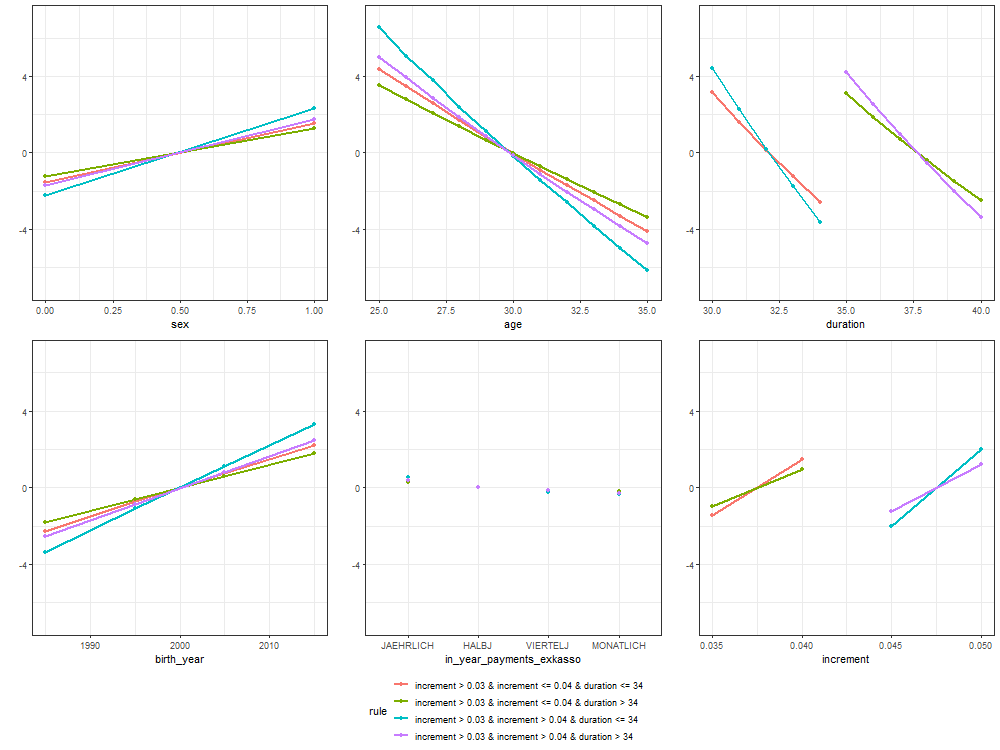
\includegraphics[width=16cm]{Figures/insurance_use_case/k1_08_BPV/effects_duration.png}
    \caption{Input-output relation of features in nodes split by duration for SLIM tree with B-splines and depth 3 (nodes 11-14)}
    \label{fig:ins_k108_effects_duration}
\end{figure}


Since increment\_factor interacts with so many features, the splits are very effective here and bring a great improvement in performance. Table \ref{tab:ins_k108_share} shows the share of the splits by the different features. From this it can be seen that MOB and CTree split shallow MBTs considerably less by increment\_factor than SLIM and GUIDE. At the same time, their performance is behind that of SLIM and GUIDE, as can be seen in Table \ref{tab:ins_k108_bsplines_surrogates_perf}. SLIM achieves the best performance.





By using deep trees, the fidelity increases and the results of the different algorithms move closer together. The values for share also get closer. Overall, the differences between the different algorithms are therefore less pronounced with the deep trees than with the shallow trees. Although the deep trees achieve a high training performance, an interpretation is hardly possible with this high number of leaf nodes. In addition, the test performance differs more strongly from the training performance than with the shallow trees, which is a sign of overfitting.



\begin{table}[!htb]

\caption{fidelity of K1\_08 B-spline baseline model and  B-spline MBTs K2204}
\centering \scriptsize
\begin{tabular}[t]{l|r|r|r|r|r|r|r|r|r}
\hline
& \multicolumn{4}{|c|}{train} & \multicolumn{4}{|c|}{test} & \\
hline
 & $R^2$ & MSE & MAE & max AE & $R^2$ & MSE & MAE & max AE & n leaves\\
\hline

B-spline & 0.927748 & 3.534102 & 1.291762 & 16.412655 & 0.927267 & 3.558816 & 1.295778 & 16.413200 & 1\\
\hline
SLIM shallow & 0.997432 & 0.125606 & 0.235344 & 4.296943 & 0.997397 & 0.127386 & 0.236761 & 4.299219 & 8\\
GUIDE shallow & 0.996540 & 0.169233 & 0.262321 & 5.006522 & 0.996496 & 0.171433 & 0.263770 & 5.003334 & 8\\
MOB shallow & 0.994944 & 0.247289 & 0.324474 & 5.236252 & 0.994942 & 0.247489 & 0.324895 & 5.336406 & 8\\
CTree shallow & 0.993049 & 0.340023 & 0.401982 & 5.236252 & 0.993055 & 0.339838 & 0.401632 & 5.336406 & 8\\
\hline
SLIM deep & 0.999882 & 0.005794 & 0.043939 & 1.079069 & 0.999870 & 0.006350 & 0.045885 & 1.126732 & 105\\
GUIDE deep & 0.999844 & 0.007652 & 0.052102 & 1.079069 & 0.999832 & 0.008219 & 0.054046 & 1.126732 & 95\\
MOB deep & 0.999861 & 0.006823 & 0.047428 & 1.079069 & 0.999848 & 0.007460 & 0.049459 & 1.126732 & 108\\
CTree deep & 0.999839 & 0.007851 & 0.058806 & 1.079069 & 0.999825 & 0.008539 & 0.061363 & 1.126732 & 106\\
\hline
\end{tabular}
\label{tab:ins_k108_bsplines_surrogates_perf}
\end{table}




\begin{table}[!htb]
\caption{Share of observations split by the different features K1\_08 B-spline MBTs}
\centering \scriptsize
\begin{tabular}[t]{l|r|r|r|r|r}
\hline
  & sex & age & duration & birth\_year & increment\\
\hline
SLIM shallow & 0.00 & 0.00 & 0.12 & 0.00  & 0.88\\
GUIDE shallow & 0.00 & 0.12 & 0.00 & 0.00  & 0.88\\
MOB shallow & 0.00 & 0.12 & 0.33 & 0.00  & 0.54\\
CTree shallow & 0.00 & 0.33 & 0.33 & 0.00  & 0.33\\
\hline
SLIM deep & 0.10 & 0.08 & 0.24 & 0.05 & 0.54\\
GUIDE deep & 0.06 & 0.10 & 0.22 & 0.05 & 0.56\\
MOB deep & 0.11 & 0.15 & 0.20 & 0.03 & 0.52\\
CTree deep & 0.00 & 0.17 & 0.29 & 0.05 & 0.49\\
\hline
\end{tabular}
\label{tab:ins_k108_share}
\end{table}

The feature payment\_period, in\_year\_payments\_exkasso and guarantee\_period are never chosen as splitting variables and are therfore not listed in the table.


As for K2204 two SLIM trees with B-spline models are fitted as  standalone models for BPV and their accuracy is compared with the black box model. The result is shown in Table \ref{tab:ins_k108_standalone_slim}. For this data set, too, the deviations are most considerable for the max ae





\begin{table}[!htb]

\caption{Accuracy of standalone B-spline SLIM MBTs and of the black box model K1\_08}
\centering \scriptsize  
\begin{tabular}[t]{l|r|r|r|r|r|r|r|r}
\hline
 & \multicolumn{4}{|c|}{train} & \multicolumn{4}{|c}{test} \\
\hline
 & $R^2$ & MSE & MAE & max AE & $R^2$ & MSE & MAE & max AE \\
\hline
SLIM shallow & 0.9974321 & 0.1256075 & 0.2353447 & 4.3046812 & 0.9973966 & 0.1273854 & 0.2367417 & 4.3074899\\
SLIM deep & 0.9998814 & 0.0057987 & 0.0439357 & 1.0862638 & 0.9998702 & 0.0063532 & 0.0458758 & 1.1344576\\
Blackbox & 1.0000000 & 0.0000023 & 0.0011006 & 0.0096827 & 1.0000000 & 0.0000023 & 0.0010968 & 0.0099144\\
\hline
\end{tabular}
\label{tab:ins_k108_standalone_slim}
\end{table}
\newpage

\clearpage


\section{Conclusion}
\label{conclusion}
In order to obtain a surrogate model that is able to partition the feature space in such a way that in the subregions main effect only models can approximate the black box model well, four different MBT algorithms were compared in this thesis.

The comparison of the selection bias showed that according to the classical definition (i.e. independence scenario) and with numerical variables only indeed only SLIM shows a selection bias, while the other methods seem to be unbiased. A correction approach to eliminate the selection bias under numerical variables in SLIM was not successful.
When adding categorical variables, however, GUIDE, MOB and CTree also showed a selection bias. If, instead of the independence scenario, scenarios were examined in which interactions were actually present, a bias was also found there for all algorithms.
This problem should always be considered when applying the algorithms without defining the roles of the features (regressor vs partitiong) in advance, as in this thesis. In extreme cases, it could lead to the phenomenon that features are chosen as splitting variables only because of their scale, although other features actually have a stronger share of interactions.

When examining the splitting behaviour of the algorithms for scenarios with two interactions of the same size with different feature types, it was notable that SLIM, GUIDE and partly also MOB choose variables for splitting that reveal subgroups much more frequently than CTree. This enables them to generate considerable smaller and yet better performing trees than CTree (and MOB), if subgroup depending main effects exist.
This was also shown in the subsequent simulations, with the aim of comparing interpretability, performance and interpretability of the different algorithms. 

As a fundamental problem of all algorithms, however, it turned out that smooth interactions can often only be modelled well by a large number of binary splits, which makes a global interpretation of MBTs difficult or even impossible for such data. In such cases, MBTs are probably not the best choice for surrogate models and models like GA2M \citep{Lou.2013} should be preferred.


One advantage that SLIM and GUIDE have over the other two algorithms is that they are more flexible in the selection of different (for example penalized) models in the nodes.
However, there is potential for improvement for SLIM and GUIDE in the area of pruning. Some simulations showed that the size of the trees varies greatly for both algorithms and that sometimes (incorrectly) highly asymmetric trees are created. To improve this, hyperparameter tuning of the prepruning parameters would be an option. For SLIM, however, this could lead to a considerable computational effort because of the exhaustive search, whereas GUIDE could be better suited for this.

The simulation example with nonlinear effects as well as the application of MBTs on insurance data sets have shown that it is recommended to use non-linear models in the leafnodes. This improves the performance considerably and also ensures that the split is actually based on interactions.
The split effects can then be interpreted visually, which was carried out in the insurance data use case.
If it is necessary that the parameter estimators of the models are directly interpretable, linear models or polynomial (penalised) models are an alternative.


MBT algorithms, especially SLIM and GUIDE, are a promising addition - although not a universal solution - to the possible model classes for surrogate models. Through the combination of decision rules and (nonlinear) main effect models, a relatively high performance and interpretability can be achieved at the same time. However, interpretability decreases very quickly with a high number of subregions. A compromise must therefore always be found here. In general, it is advisable to use different IML methods simultaneously to check the plausibility of the individual results or to compare them with expert knowledge, which was done in the case of the insurance data sets.



\newpage





\newpage
  
\pagenumbering{Roman}
%\setcounter{page}{4} % CHANGE
% ------------------------------------------------------------------------------
% BIBLIOGRAPHY -----------------------------------------------------------------
% ------------------------------------------------------------------------------

\bibliography{bibliography}
\bibliographystyle{dcu}
\newpage
\newpage
\listoffigures
\newpage
\listoftables
\newpage

% ------------------------------------------------------------------------------
% APPENDIX ---------------------------------------------------------------------
% ------------------------------------------------------------------------------
\appendix

\section{Appendix}
\label{app}
\subsection{GUIDE implementation results}

\subsection{Selection Bias correction approach SLIM}

By means of a simulation, I investigated how the number of quantiles (n.quantiles) used as potential splitpoints in SLIM affects the selection bias for numerical features. 
The data is defined as follows:
\begin{itemize}
    \item $\textbf{x}_1, \textbf{x}_2 \sim U(0,1)$
    \item $\textbf{x}_3$ uniformly distributed on equidistant grids of length 10, 25, 50 and 100 on the interval [0,1] (i.e. four different settings)
    \item $y \sim N(0,1)$
\end{itemize}

For each of the four simulation scenarios, SLIM trees are fitted  with  \\ n.quantiles $\in \{100, 75, 50, 25, 10, 2\}$ and one exact tree (each unique value as potential splitpoint) in each simulation run. The experiment is repeated 1000 times.

To measure whether and how the selection bias improves, a $\chi^2$ goodness of fit test is used. The null hypothesis is that the probability of all three features being selected as splitting variable is equal. To compare the results, the p-value of the tests are used. The p-value gives the probability that the null hypothesis of unbiasedness of the split variables in the first split is falsely rejected. I.e. a small p-value is a sign of selection bias, while a high p-value means that the null hypothesis of unbiasedness is not rejected.

In addition to p-value, the mean squared error is measured on the test and on the training data.

Figure \ref{fig:app_selection_bias_slim} shows the results of the four variants

\begin{figure}[!htb]
    \centering
    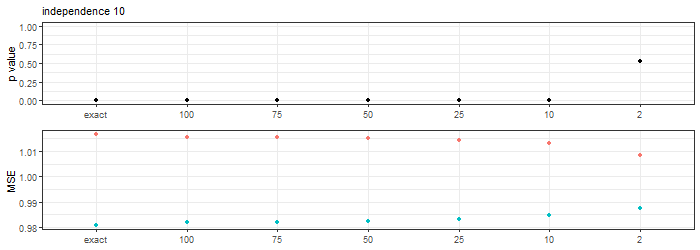
\includegraphics[width = 12cm]{Figures/simulations/batchtools/selection_bias_slim/independence_10.png}\\
    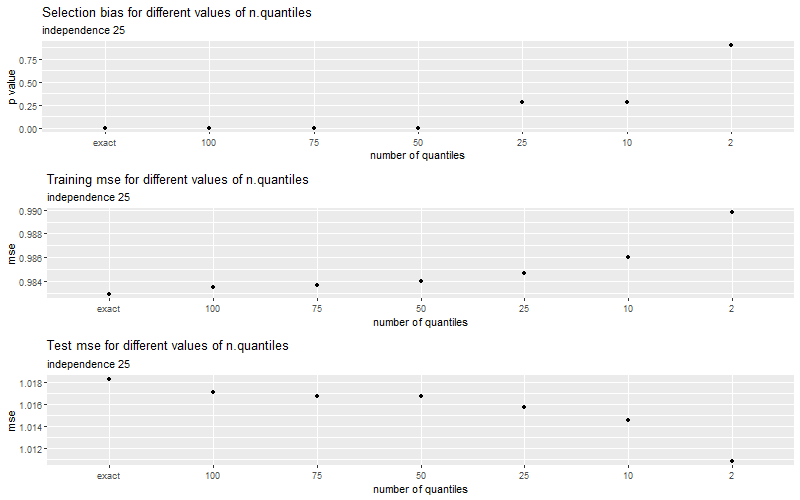
\includegraphics[width = 12cm]{Figures/simulations/batchtools/selection_bias_slim/independence_25.png}\\
    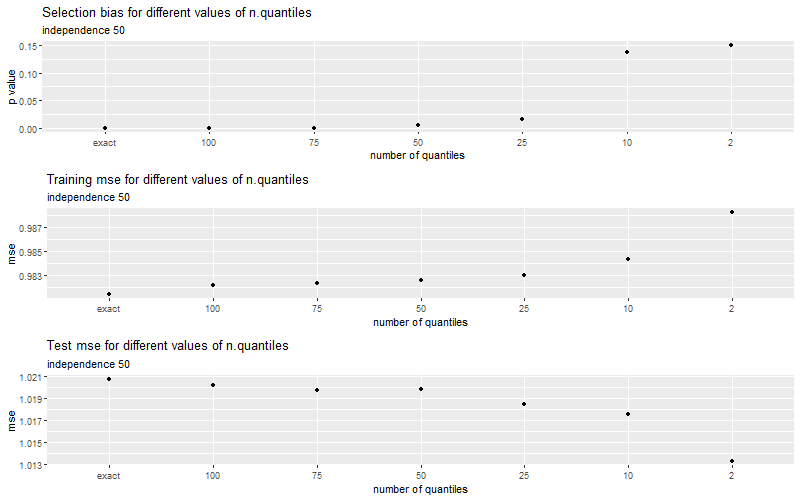
\includegraphics[width = 12cm]{Figures/simulations/batchtools/selection_bias_slim/independence_50.png}\\
    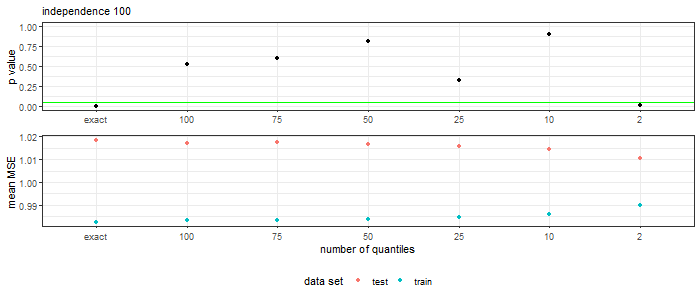
\includegraphics[width = 12cm]{Figures/simulations/batchtools/selection_bias_slim/independence_100.png}\\
    \caption{impact of the value of n.quantiles on selection bias and performance}
    \label{fig:app_selection_bias_slim}
\end{figure}



\clearpage
\subsection{Simulation results}
\subsubsection{Basic scenarios}
\begin{table}[!htb]

\caption{Mean simulation results on 100 simulation runs as surrogate models on scenario \textbf{linear smooth} with sample size $n = 1500$ for different values of impr and alpha}
\centering \tiny
\begin{tabular}[t]{l|l|r|r|r|r|r|r|r|r|r}
\hline
black box & MBT & impr & alpha & n leaves & n leaves min & n leaves max &  $R^2_{train}$ & sd $R^2_{train}$ & $R^2_{test}$ & sd $R^2_{test}$\\
\hline
lm & SLIM & 0.15 & & 2.06 & 2 & 3 & 0.9650 & 0.0043 & 0.9631 & 0.0046\\
lm & SLIM & 0.10 & & 12.11 & 5 & 16 & 0.9965 & 0.0052 & 0.9958 & 0.0060\\
lm & SLIM & 0.05 & & 15.70 & 14 & 16 & 0.9995 & 0.0001 & 0.9993 & 0.0001\\
lm & GUIDE & 0.15 & & 2.07 & 2 & 3 & 0.9651 & 0.0044 & 0.9632 & 0.0049\\
lm & GUIDE & 0.10 & & 12.03 & 5 & 16 & 0.9965 & 0.0051 & 0.9957 & 0.0060\\
lm & GUIDE & 0.05 & & 15.75 & 14 & 16 & 0.9995 & 0.0001 & 0.9993 & 0.0001\\
lm & MOB & & 0.001 & 15.78 & 14 & 16 & 0.9994 & 0.0001 & 0.9993 & 0.0001\\
lm & MOB & & 0.010 & 15.78 & 14 & 16 & 0.9994 & 0.0001 & 0.9993 & 0.0001\\
lm & MOB & & 0.050 & 15.78 & 14 & 16 & 0.9994 & 0.0001 & 0.9993 & 0.0001\\
lm & CTree & & 0.001 & 15.22 & 13 & 17 & 0.9993 & 0.0001 & 0.9992 & 0.0001\\
lm & CTree & & 0.010 & 15.22 & 13 & 17 & 0.9993 & 0.0001 & 0.9992 & 0.0001\\
lm & CTree & & 0.050 & 15.22 & 13 & 17 & 0.9993 & 0.0001 & 0.9992 & 0.0001\\
\hline
lm &  & & & & &  & 0.9902 & 0.0006 & 0.9901 & 0.0008\\
\hline

xgboost & SLIM & 0.15 & & 2.31 & 2 & 6 & 0.9665 & 0.0069 & 0.9629 & 0.0079\\
xgboost & SLIM & 0.10 & & 7.33 & 2 & 14 & 0.9850 & 0.0060 & 0.9814 & 0.0062\\
xgboost & SLIM & 0.05 & & 14.30 & 8 & 17 & 0.9948 & 0.0010 & 0.9909 & 0.0017\\
xgboost & GUIDE & 0.15 & & 2.26 & 2 & 5 & 0.9664 & 0.0067 & 0.9628 & 0.0077\\
xgboost & GUIDE & 0.10 & & 6.92 & 2 & 14 & 0.9847 & 0.0061 & 0.9811 & 0.0062\\
xgboost & GUIDE & 0.05 & & 14.15 & 8 & 17 & 0.9945 & 0.0010 & 0.9906 & 0.0017\\
xgboost & MOB & & 0.001 & 10.89 & 8 & 13 & 0.9944 & 0.0005 & 0.9904 & 0.0011\\
xgboost & MOB & & 0.010 & 11.96 & 9 & 15 & 0.9946 & 0.0005 & 0.9906 & 0.0011\\
xgboost & MOB & & 0.050 & 12.86 & 11 & 15 & 0.9948 & 0.0005 & 0.9908 & 0.0011\\
xgboost & CTree & & 0.001 & 12.09 & 9 & 15 & 0.9940 & 0.0006 & 0.9900 & 0.0012\\
xgboost & CTree & & 0.010 & 13.21 & 10 & 15 & 0.9943 & 0.0006 & 0.9902 & 0.0013\\
xgboost & CTree & & 0.050 & 14.09 & 11 & 17 & 0.9944 & 0.0006 & 0.9904 & 0.0012\\
\hline
xgboost &  & & &  &  &  & 0.9858 & 0.0008 & 0.9768 & 0.0018\\
\hline
\end{tabular}
\label{tab:app_linear_smooth_1000}
\end{table}


\begin{figure}[!htb]
\caption{Maximum leaf size of standalone MBTs vs number of leaf nodes scenario linear smooth with $n=1500, alpha = 0.001, impr = 0.1$}
    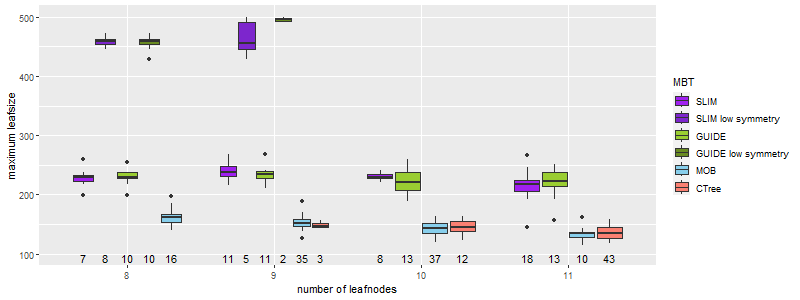
\includegraphics[width=16cm]{Figures/simulations/batchtools/basic_scenarios/linear_smooth/ls_1000_standalone_symmetrie.png}
    \label{fig:app_ls_1000_standalone_symmetrie}
\end{figure} 


\begin{figure}[!htb]
\caption{Test fidelity $R^2$ as surrogate on lm predictions vs number of leaf nodes scenario linear smooth with $n=1500, alpha = 0.001, impr = 0.1$}
    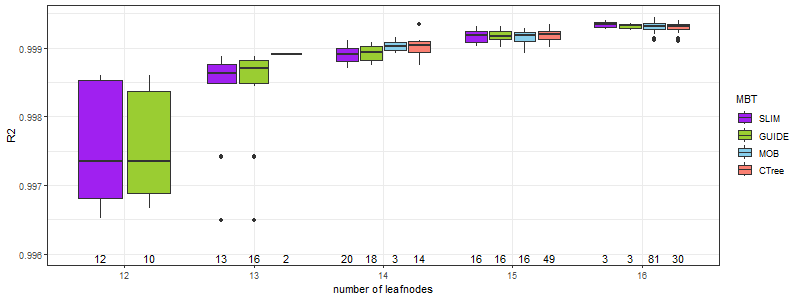
\includegraphics[width=16cm]{Figures/simulations/batchtools/basic_scenarios/linear_smooth/ls_1000_lm_r2_test.png}
    \label{fig:app_ls_1000_lm_r2_test}
\end{figure} 

\begin{figure}[!htb]
\caption{Test fidelity $R^2$ as surrogate on xgboost predictions vs number of leaf nodes scenario linear smooth with $n=1500, alpha = 0.001, impr = 0.1$}
    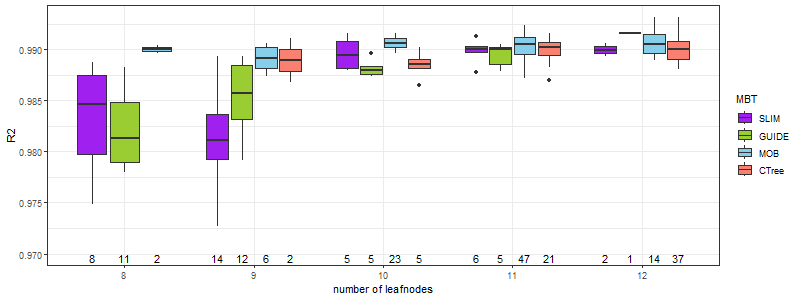
\includegraphics[width=16cm]{Figures/simulations/batchtools/basic_scenarios/linear_smooth/ls_1000_xgboost_r2_test.png}
    \label{fig:app_ls_1000_xgboost_r2_test}
\end{figure} 



\begin{table}[!htb]

\caption{Mean simulation results on 100 simulation runs as stand alone and surrogate models on scenario \textbf{linear smooth} with sample size n = 5000 for different values of $impr$ and $alpha$}
\centering \tiny
\begin{tabular}[t]{l|l|r|r|r|r|r|r|r|r|r}
\hline
black box & MBT & impr & alpha & n leaves & n leaves min & n leaves max &  $R^2_{train}$ & sd $R^2_{train}$ & $R^2_{test}$ & sd $R^2_{test}$\\

\hline

standalone & SLIM & 0.15 & & 2.04 & 2 & 3 & 0.9542 & 0.0034 & 0.9536 & 0.0036\\
standalone & SLIM & 0.10 & & 36.94 & 15 & 58 & 0.9895 & 0.0024 & 0.9880 & 0.0024\\
standalone & SLIM & 0.05 & & 55.84 & 50 & 61 & 0.9910 & 0.0002 & 0.9890 & 0.0004\\
standalone & GUIDE & 0.15 & & 2.03 & 2 & 3 & 0.9540 & 0.0030 & 0.9534 & 0.0031\\
standalone & GUIDE & 0.10 & & 36.23 & 14 & 52 & 0.9894 & 0.0023 & 0.9881 & 0.0024\\
standalone & GUIDE & 0.05 & & 56.35 & 47 & 62 & 0.9909 & 0.0002 & 0.9891 & 0.0003\\
standalone & MOB & & 0.001 & 17.15 & 16 & 21 & 0.9901 & 0.0002 & 0.9893 & 0.0004\\
standalone & MOB & & 0.010 & 19.14 & 16 & 22 & 0.9902 & 0.0002 & 0.9894 & 0.0004\\
standalone & MOB & & 0.050 & 21.71 & 18 & 26 & 0.9903 & 0.0002 & 0.9895 & 0.0004\\
standalone & CTree & & 0.001 & 19.19 & 17 & 22 & 0.9901 & 0.0002 & 0.9894 & 0.0004\\
standalone & CTree &0 & 0.010 & 21.58 & 17 & 25 & 0.9902 & 0.0002 & 0.9895 & 0.0004\\
standalone & CTree & & 0.050 & 24.56 & 21 & 30 & 0.9903 & 0.0002 & 0.9895 & 0.0003\\


\hline
lm & SLIM & 0.15 & & 2.00 & 2 & 2 & 0.9628 & 0.0009 & 0.9625 & 0.0012\\
lm & SLIM & 0.10 & & 52.19 & 43 & 60 & 0.9999 & 0.0001 & 0.9998 & 0.0001\\
lm & SLIM & 0.05 & & 63.99 & 63 & 64 & 1.0000 & 0.0000 & 1.0000 & 0.0000\\
lm & GUIDE & 0.15 &  & 2.00 & 2 & 2 & 0.9628 & 0.0009 & 0.9625 & 0.0012\\
lm & GUIDE & 0.10 &  & 52.37 & 43 & 60 & 0.9999 & 0.0001 & 0.9998 & 0.0001\\
lm & GUIDE & 0.05 & & 63.99 & 63 & 64 & 1.0000 & 0.0000 & 1.0000 & 0.0000\\
lm & MOB & & 0.001 & 64.00 & 64 & 64 & 1.0000 & 0.0000 & 1.0000 & 0.0000\\
lm & MOB & & 0.010 & 64.00 & 64 & 64 & 1.0000 & 0.0000 & 1.0000 & 0.0000\\
lm & MOB & & 0.050 & 64.00 & 64 & 64 & 1.0000 & 0.0000 & 1.0000 & 0.0000\\
lm & CTree & & 0.001 & 63.60 & 62 & 64 & 1.0000 & 0.0000 & 1.0000 & 0.0000\\
lm & CTree & & 0.010 & 63.60 & 62 & 64 & 1.0000 & 0.0000 & 1.0000 & 0.0000\\
lm & CTree &5 & 0.050 & 63.60 & 62 & 64 & 1.0000 & 0.0000 & 1.0000 & 0.0000\\
\hline
lm & & & & & & & 0.9901 & 0.0002 & 0.9901 & 0.0003\\
\hline



xgboost & SLIM & 0.15 & & 2.22 & 2 & 7 & 0.9647 & 0.0063 & 0.9643 & 0.0063\\
xgboost & SLIM & 0.10 & & 19.23 & 3 & 40 & 0.9908 & 0.0062 & 0.9902 & 0.0062\\
xgboost & SLIM & 0.05 & & 49.05 & 34 & 56 & 0.9978 & 0.0003 & 0.9972 & 0.0003\\
xgboost & CTree & 0.15 & & 32.81 & 26 & 41 & 0.9972 & 0.0002 & 0.9965 & 0.0003\\
xgboost & CTree & 0.10 & & 36.36 & 29 & 43 & 0.9973 & 0.0002 & 0.9966 & 0.0003\\
xgboost & CTree & 0.05 & & 39.37 & 32 & 47 & 0.9974 & 0.0002 & 0.9967 & 0.0003\\
xgboost & MOB & & 0.001 & 38.44 & 29 & 47 & 0.9979 & 0.0002 & 0.9972 & 0.0003\\
xgboost & MOB & & 0.010 & 42.62 & 31 & 53 & 0.9980 & 0.0002 & 0.9973 & 0.0003\\
xgboost & MOB & & 0.050 & 46.02 & 39 & 55 & 0.9981 & 0.0002 & 0.9974 & 0.0003\\
xgboost & GUIDE & & 0.001 & 2.21 & 2 & 8 & 0.9645 & 0.0061 & 0.9641 & 0.0062\\
xgboost & GUIDE & & 0.010 & 19.27 & 3 & 38 & 0.9907 & 0.0062 & 0.9900 & 0.0062\\
xgboost & GUIDE & & 0.050 & 49.90 & 34 & 58 & 0.9977 & 0.0003 & 0.9970 & 0.0004\\
\hline
xgboost & & & & & & & 0.9877 & 0.0003 & 0.9852 & 0.0006\\
\hline

\hline
\end{tabular}
\label{tab:app_linear_smooth_5000}

\end{table}



\begin{table}[!htb]

\caption{Mean simulation results on 100 simulation runs as surrogate models  on scenario \textbf{linear categorical} with sample size n=1500 for different values of impr and alpha}
\centering \tiny
\begin{tabular}[t]{l|l|r|r|r|r|r|r|r|r|r}
\hline
black box & MBT & impr & alpha & n leaves & n leaves min & n leaves max &  $R^2_{train}$ & sd $R^2_{train}$ & $R^2_{test}$ & sd $R^2_{test}$\\
\hline
gam & SLIM & 0.15 & & 2.00 & 2 & 2 & 0.8528 & 0.0064 & 0.8513 & 0.0108\\
gam & SLIM & 0.10 & & 2.64 & 2 & 4 & 0.8972 & 0.0432 & 0.8937 & 0.0440\\
gam & SLIM & 0.05 & & 8.56 & 4 & 16 & 0.9910 & 0.0029 & 0.9893 & 0.0039\\
gam & GUIDE & 0.15 & & 2.00 & 2 & 2 & 0.8528 & 0.0064 & 0.8513 & 0.0108\\
gam & GUIDE & 0.10 & & 2.64 & 2 & 4 & 0.8972 & 0.0432 & 0.8937 & 0.0440\\
gam & GUIDE & 0.05 & & 6.06 & 4 & 13 & 0.9875 & 0.0031 & 0.9859 & 0.0038\\
gam & MOB & & 0.001 & 13.53 & 11 & 15 & 0.9773 & 0.0020 & 0.9718 & 0.0028\\
gam & MOB & & 0.010 & 14.28 & 13 & 16 & 0.9784 & 0.0020 & 0.9728 & 0.0029\\
gam & MOB & & 0.050 & 14.92 & 13 & 16 & 0.9797 & 0.0021 & 0.9740 & 0.0028\\
gam & CTree & & 0.001 & 13.89 & 11 & 16 & 0.9773 & 0.0018 & 0.9720 & 0.0028\\
gam & CTree & & 0.010 & 14.47 & 12 & 16 & 0.9779 & 0.0017 & 0.9725 & 0.0027\\
gam & CTree & & 0.050 & 14.86 & 13 & 16 & 0.9783 & 0.0016 & 0.9729 & 0.0028\\
\hline
gam & & & & & & & 0.9702 & 0.0018 & 0.9694 & 0.0029\\
\hline

xgboost & SLIM & 0.15 & & 2.00 & 2 & 2 & 0.8321 & 0.0075 & 0.8323 & 0.0118\\
xgboost & SLIM & 0.10 & & 4.00 & 4 & 4 & 0.9923 & 0.0012 & 0.9870 & 0.0029\\
xgboost & SLIM & 0.05 & & 4.00 & 4 & 4 & 0.9923 & 0.0012 & 0.9870 & 0.0029\\
xgboost & GUIDE & 0.15 & & 2.00 & 2 & 2 & 0.8321 & 0.0075 & 0.8323 & 0.0118\\
xgboost & GUIDE & 0.10 & & 4.00 & 4 & 4 & 0.9923 & 0.0012 & 0.9870 & 0.0029\\
xgboost & GUIDE & 0.05 & & 4.00 & 4 & 4 & 0.9923 & 0.0012 & 0.9870 & 0.0029\\
xgboost & MOB & & 0.001 & 13.45 & 11 & 16 & 0.9793 & 0.0063 & 0.9729 & 0.0069\\
xgboost & MOB & & 0.010 & 14.38 & 13 & 16 & 0.9831 & 0.0055 & 0.9765 & 0.0066\\
xgboost & MOB & & 0.050 & 14.63 & 13 & 16 & 0.9837 & 0.0052 & 0.9771 & 0.0062\\
xgboost & CTree & & 0.001 & 11.96 & 10 & 14 & 0.9602 & 0.0030 & 0.9545 & 0.0049\\
xgboost & CTree & & 0.010 & 12.76 & 10 & 15 & 0.9612 & 0.0033 & 0.9550 & 0.0050\\
xgboost & CTree & & 0.050 & 13.46 & 10 & 16 & 0.9623 & 0.0036 & 0.9558 & 0.0052\\
\hline
xgboost & & & & & & & 0.9876 & 0.0015 & 0.9778 & 0.0031\\
\hline
\end{tabular}
\label{tab:app_linear_abrupt_1000}

\end{table}



\begin{table}[!htb]

\caption{Mean simulation results on 100 simulation runs as stand alone and surrogate models on scenario \textbf{linear categorical} with sample size n = 5000 for different values of impr and alpha}
\centering \tiny
\begin{tabular}[t]{l|l|r|r|r|r|r|r|r|r|r}
\hline
black box & MBT & impr & alpha & n leaves & n leaves min & n leaves max &  $R^2_{train}$ & sd $R^2_{train}$ & $R^2_{test}$ & sd $R^2_{test}$\\
\hline
standalone & SLIM & 0.15 & & 2.00 & 2 & 2 & 0.8277 & 0.0032 & 0.8267 & 0.0048\\
standalone & SLIM & 0.10 & & 4.00 & 4 & 4 & 0.9887 & 0.0008 & 0.9886 & 0.0011\\
standalone & SLIM & 0.05 & & 4.00 & 4 & 4 & 0.9887 & 0.0008 & 0.9886 & 0.0011\\
standalone & GUIDE & 0.15 & & 2.00 & 2 & 2 & 0.8277 & 0.0032 & 0.8267 & 0.0048\\
standalone & GUIDE & 0.10 & & 4.00 & 4 & 4 & 0.9887 & 0.0008 & 0.9886 & 0.0011\\
standalone & GUIDE & 0.05 & & 4.00 & 4 & 4 & 0.9887 & 0.0008 & 0.9886 & 0.0011\\
standalone & MOB & & 0.001 & 41.23 & 26 & 48 & 0.9896 & 0.0004 & 0.9868 & 0.0011\\
standalone & MOB & & 0.010 & 45.50 & 27 & 53 & 0.9899 & 0.0003 & 0.9871 & 0.0011\\
standalone & MOB & & 0.050 & 49.24 & 31 & 58 & 0.9902 & 0.0003 & 0.9874 & 0.0011\\
standalone & CTree & & 0.001 & 22.51 & 20 & 25 & 0.9499 & 0.0014 & 0.9462 & 0.0022\\
standalone & CTree & & 0.010 & 24.39 & 21 & 27 & 0.9502 & 0.0014 & 0.9464 & 0.0023\\
standalone & CTree & & 0.050 & 26.62 & 22 & 30 & 0.9507 & 0.0016 & 0.9468 & 0.0023\\

\hline
gam & SLIM & 0.15 & & 2.00 & 2 & 2 & 0.8532 & 0.0029 & 0.8527 & 0.0043\\
gam & SLIM & 0.10 & & 2.22 & 2 & 4 & 0.8681 & 0.0299 & 0.8668 & 0.0302\\
gam & SLIM & 0.05 & & 27.66 & 13 & 42 & 0.9940 & 0.0036 & 0.9935 & 0.0039\\
gam & GUIDE & 0.15 & & 2.00 & 2 & 2 & 0.8532 & 0.0029 & 0.8527 & 0.0043\\
gam & GUIDE & 0.10 & & 2.22 & 2 & 4 & 0.8681 & 0.0299 & 0.8668 & 0.0302\\
gam & GUIDE & 0.05 & & 14.56 & 4 & 31 & 0.9886 & 0.0038 & 0.9882 & 0.0040\\
gam & MOB & & 0.001 & 61.11 & 55 & 64 & 0.9973 & 0.0002 & 0.9966 & 0.0003\\
gam & MOB & & 0.010 & 62.42 & 59 & 64 & 0.9973 & 0.0002 & 0.9966 & 0.0002\\
gam & MOB & & 0.050 & 63.15 & 61 & 64 & 0.9974 & 0.0002 & 0.9967 & 0.0002\\
gam & CTree & & 0.001 & 33.93 & 31 & 38 & 0.9789 & 0.0007 & 0.9769 & 0.0011\\
gam & CTree & & 0.010 & 36.76 & 34 & 43 & 0.9793 & 0.0008 & 0.9772 & 0.0012\\
gam & CTree & & 0.050 & 39.43 & 36 & 45 & 0.9798 & 0.0010 & 0.9776 & 0.0013\\

\hline
gam & & & & & & & 0.9701 & 0.0010 & 0.9698 & 0.0014\\
\hline

xgboost & SLIM & 0.15 & & 2.00 & 2 & 2 & 0.8335 & 0.0033 & 0.8334 & 0.0048\\
xgboost & SLIM & 0.10 & & 4.00 & 4 & 4 & 0.9949 & 0.0009 & 0.9942 & 0.0011\\
xgboost & SLIM & 0.05 & & 4.00 & 4 & 4 & 0.9949 & 0.0009 & 0.9942 & 0.0011\\
xgboost & GUIDE & 0.15 & & 2.00 & 2 & 2 & 0.8335 & 0.0033 & 0.8334 & 0.0048\\
xgboost & GUIDE & 0.10 & & 4.00 & 4 & 4 & 0.9949 & 0.0009 & 0.9942 & 0.0011\\
xgboost & GUIDE & 0.05 & & 4.00 & 4 & 4 & 0.9949 & 0.0009 & 0.9942 & 0.0011\\
xgboost & MOB & & 0.001 & 53.91 & 49 & 60 & 0.9987 & 0.0002 & 0.9974 & 0.0007\\
xgboost & MOB & & 0.010 & 55.38 & 49 & 60 & 0.9988 & 0.0002 & 0.9974 & 0.0007\\
xgboost & MOB & & 0.050 & 56.40 & 50 & 61 & 0.9988 & 0.0002 & 0.9974 & 0.0007\\
xgboost & CTree & & 0.001 & 24.16 & 19 & 29 & 0.9600 & 0.0016 & 0.9577 & 0.0021\\
xgboost & CTree &  & 0.010 & 26.39 & 21 & 32 & 0.9605 & 0.0015 & 0.9581 & 0.0021\\
xgboost & CTree & & 0.050 & 28.97 & 22 & 36 & 0.9612 & 0.0017 & 0.9587 & 0.0023\\
\hline
xgboost & & & & & & & 0.9880 & 0.0009 & 0.9852 & 0.0009\\
\hline

\end{tabular}
\label{tab:app_linear_abrupt_5000}

\end{table}




\begin{table}[!htb]

\caption{Mean simulation results on 100 simulation runs as surrogate models on scenario \textbf{linear mixed} with sample size $n=1500$ for different values of impr and alpha}
\centering \tiny
\begin{tabular}[t]{l|l|r|r|r|r|r|r|r|r|r}
\hline
black box & MBT & impr & alpha & n leaves & n leaves min & n leaves max &  $R^2_{train}$ & sd $R^2_{train}$ & $R^2_{test}$ & sd $R^2_{test}$\\
\hline
lm & SLIM & 0.15 & & 3.20 & 2 & 13 & 0.8879 & 0.0309 & 0.8806 & 0.0331\\
lm & SLIM & 0.10 & & 13.07 & 5 & 16 & 0.9875 & 0.0098 & 0.9843 & 0.0108\\
lm & SLIM & 0.05 & & 14.78 & 12 & 16 & 0.9913 & 0.0020 & 0.9885 & 0.0028\\
lm & GUIDE & 0.15 & & 3.17 & 2 & 13 & 0.8872 & 0.0308 & 0.8799 & 0.0329\\
lm & GUIDE & 0.10 & & 12.66 & 7 & 16 & 0.9866 & 0.0095 & 0.9834 & 0.0106\\
lm & GUIDE & 0.05 & & 14.38 & 12 & 16 & 0.9905 & 0.0022 & 0.9876 & 0.0029\\
lm & MOB & & 0.001 & 14.99 & 13 & 17 & 0.9882 & 0.0016 & 0.9838 & 0.0021\\
lm & MOB & & 0.010 & 14.99 & 13 & 17 & 0.9882 & 0.0016 & 0.9838 & 0.0021\\
lm & MOB & & 0.050 & 14.99 & 13 & 17 & 0.9882 & 0.0016 & 0.9838 & 0.0021\\
lm & CTree & & 0.001 & 15.05 & 13 & 17 & 0.9880 & 0.0016 & 0.9841 & 0.0019\\
lm & CTree & & 0.010 & 15.05 & 13 & 17 & 0.9880 & 0.0016 & 0.9841 & 0.0019\\
lm & CTree & & 0.050 & 15.05 & 13 & 17 & 0.9880 & 0.0016 & 0.9841 & 0.0019\\

\hline
lm & & & & & & & 0.9902 & 0.0006 & 0.9898 & 0.0008\\
\hline


xgboost & SLIM & 0.15 & & 4.47 & 2 & 13 & 0.9067 & 0.0336 & 0.9013 & 0.0339\\
xgboost & SLIM & 0.10 & & 12.80 & 7 & 16 & 0.9832 & 0.0089 & 0.9724 & 0.0103\\
xgboost & SLIM & 0.05 & & 14.80 & 12 & 17 & 0.9870 & 0.0018 & 0.9764 & 0.0044\\
xgboost & GUIDE & 0.15 & & 4.37 & 2 & 13 & 0.9059 & 0.0335 & 0.9005 & 0.0339\\
xgboost & GUIDE & 0.10 & & 12.48 & 6 & 16 & 0.9822 & 0.0098 & 0.9715 & 0.0112\\
xgboost & GUIDE & 0.05 & & 14.47 & 12 & 17 & 0.9863 & 0.0022 & 0.9758 & 0.0047\\
xgboost & MOB & & 0.001 & 14.82 & 13 & 17 & 0.9853 & 0.0018 & 0.9745 & 0.0047\\
xgboost & MOB & & 0.010 & 14.94 & 13 & 17 & 0.9854 & 0.0017 & 0.9746 & 0.0046\\
xgboost & MOB & & 0.050 & 14.94 & 13 & 17 & 0.9854 & 0.0017 & 0.9746 & 0.0046\\
xgboost & CTree & & 0.001 & 15.03 & 13 & 17 & 0.9850 & 0.0017 & 0.9743 & 0.0042\\
xgboost & CTree & & 0.010 & 15.07 & 13 & 17 & 0.9850 & 0.0017 & 0.9743 & 0.0042\\
xgboost & CTree & & 0.050 & 15.07 & 13 & 17 & 0.9850 & 0.0017 & 0.9743 & 0.0042\\
\hline
xgboost & & & & & & & 0.9859 & 0.0014 & 0.9682 & 0.0042\\
\hline
\end{tabular}
\label{tab:app_linear_mixed_1000}

\end{table}





\begin{table}[!htb]

\caption{Mean simulation results on 100 simulation runs as stand alone and surrogate models on scenario \textbf{linear mixed} with sample size n = 5000 for different values of impr and alpha}
\centering \tiny
\begin{tabular}[t]{l|l|r|r|r|r|r|r|r|r|r}
\hline
black box & MBT & impr & alpha & n leaves & n leaves min & n leaves max &  $R^2_{train}$ & sd $R^2_{train}$ & $R^2_{test}$ & sd $R^2_{test}$\\
\hline
standalone & SLIM & 0.15 & & 2.30 & 2 & 8 & 0.8637 & 0.0165 & 0.8626 & 0.0176\\
standalone & SLIM & 0.10 & & 38.96 & 21 & 54 & 0.9865 & 0.0029 & 0.9849 & 0.0030\\
standalone & SLIM & 0.05 & & 59.03 & 51 & 64 & 0.9904 & 0.0005 & 0.9884 & 0.0006\\
standalone & GUIDE & 0.15 & & 2.30 & 2 & 8 & 0.8637 & 0.0165 & 0.8626 & 0.0176\\
standalone & GUIDE & 0.10 & & 38.06 & 21 & 54 & 0.9866 & 0.0028 & 0.9851 & 0.0029\\
standalone & GUIDE & 0.05 & & 58.20 & 45 & 63 & 0.9903 & 0.0005 & 0.9885 & 0.0006\\
standalone & MOB & & 0.001 & 48.54 & 43 & 55 & 0.9888 & 0.0004 & 0.9861 & 0.0007\\
standalone & MOB & & 0.010 & 53.17 & 48 & 58 & 0.9891 & 0.0003 & 0.9864 & 0.0007\\
standalone & MOB & & 0.050 & 56.07 & 51 & 60 & 0.9893 & 0.0003 & 0.9866 & 0.0006\\
standalone & CTree & & 0.001 & 51.70 & 47 & 57 & 0.9887 & 0.0004 & 0.9858 & 0.0006\\
standalone & CTree & & 0.010 & 54.85 & 50 & 58 & 0.9889 & 0.0004 & 0.9860 & 0.0006\\
standalone & CTree & & 0.050 & 56.76 & 52 & 61 & 0.9890 & 0.0003 & 0.9860 & 0.0006\\

\hline
lm & SLIM & 0.15 & & 2.17 & 2 & 16 & 0.8683 & 0.0094 & 0.8677 & 0.0103\\
lm & SLIM & 0.10 & & 39.69 & 19 & 55 & 0.9956 & 0.0028 & 0.9953 & 0.0030\\
lm & SLIM & 0.05 & & 57.51 & 46 & 64 & 0.9991 & 0.0005 & 0.9990 & 0.0006\\
lm & GUIDE & 0.15 & & 2.17 & 2 & 16 & 0.8683 & 0.0094 & 0.8677 & 0.0103\\
lm & GUIDE & 0.10 & & 40.32 & 19 & 55 & 0.9960 & 0.0026 & 0.9956 & 0.0028\\
lm & GUIDE & 0.05 & & 57.32 & 46 & 64 & 0.9991 & 0.0005 & 0.9990 & 0.0006\\
lm & MOB & & 0.001 & 63.11 & 60 & 64 & 0.9973 & 0.0002 & 0.9964 & 0.0003\\
lm & MOB & & 0.010 & 63.11 & 60 & 64 & 0.9973 & 0.0002 & 0.9964 & 0.0003\\
lm & MOB & & 0.050 & 63.11 & 60 & 64 & 0.9973 & 0.0002 & 0.9964 & 0.0003\\
lm & CTree & & 0.001 & 62.72 & 59 & 64 & 0.9973 & 0.0002 & 0.9964 & 0.0003\\
lm & CTree & & 0.010 & 62.72 & 59 & 64 & 0.9973 & 0.0002 & 0.9964 & 0.0003\\
lm & CTree & & 0.050 & 62.72 & 59 & 64 & 0.9973 & 0.0002 & 0.9964 & 0.0003\\
\hline
lm & & & & & & & 0.9901 & 0.0003 & 0.9902 & 0.0004\\
\hline


\hline
xgboost & SLIM & 0.15 & & 2.22 & 2 & 12 & 0.8693 & 0.0121 & 0.8706 & 0.0129\\
xgboost & SLIM & 0.10 & & 39.52 & 23 & 53 & 0.9931 & 0.0027 & 0.9914 & 0.0027\\
xgboost & SLIM & 0.05 & & 56.86 & 46 & 63 & 0.9964 & 0.0005 & 0.9948 & 0.0007\\
xgboost & GUIDE & 0.15 & & 2.15 & 2 & 9 & 0.8693 & 0.0119 & 0.8705 & 0.0127\\
xgboost & GUIDE & 0.10 & & 38.13 & 22 & 52 & 0.9928 & 0.0027 & 0.9912 & 0.0028\\
xgboost & GUIDE & 0.05 & & 56.72 & 46 & 63 & 0.9963 & 0.0006 & 0.9946 & 0.0007\\
xgboost & MOB & & 0.001 & 58.76 & 54 & 63 & 0.9961 & 0.0003 & 0.9942 & 0.0005\\
xgboost & MOB & & 0.010 & 59.47 & 55 & 64 & 0.9961 & 0.0003 & 0.9943 & 0.0005\\
xgboost & MOB & & 0.050 & 59.69 & 55 & 64 & 0.9961 & 0.0003 & 0.9943 & 0.0005\\
xgboost & CTree & & 0.001 & 58.51 & 53 & 62 & 0.9956 & 0.0003 & 0.9936 & 0.0005\\
xgboost & CTree & & 0.010 & 58.95 & 54 & 63 & 0.9956 & 0.0003 & 0.9936 & 0.0005\\
xgboost & CTree & & 0.050 & 59.09 & 54 & 63 & 0.9956 & 0.0003 & 0.9936 & 0.0005\\
\hline
xgboost & & & & & & & 0.9877 & 0.0007 & 0.9836 & 0.0011\\
\hline

\end{tabular}
\label{tab:app_linear_mixed_5000}

\end{table}


\clearpage
\subsubsection{Correlated features}

\subsubsection{Linear smooth with noise features}

\begin{figure}[!htb]
\caption{Test accuracy $R^2$ of MBTs on scenario Linear smooth with noise features with $n=2000, alpha = 0.001, impr = 0.1$ with $n leaves \geq 11$}
    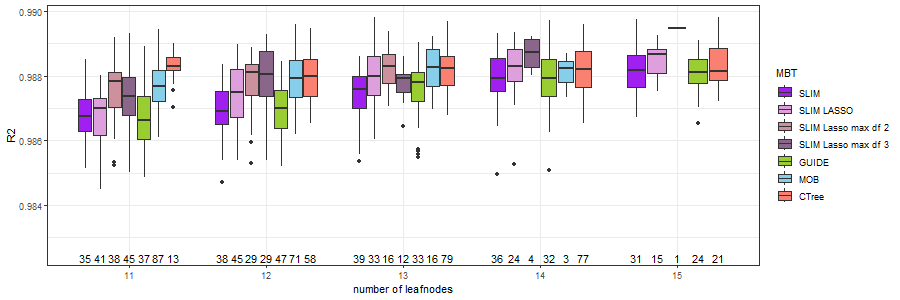
\includegraphics[width=16cm]{Figures/simulations/batchtools/lasso/lasso_standalone_r2_test.png}
    \label{fig:app_lasso_standalone_r2_test}
\end{figure} 

\begin{figure}[!htb]
\caption{Test accuracy $R^2$ of SLIM and GUIDE MBTs on scenario Linear smooth with noise features with $n=2000, alpha = 0.001, impr = 0.1$ with $n leaves \leq 11$}
    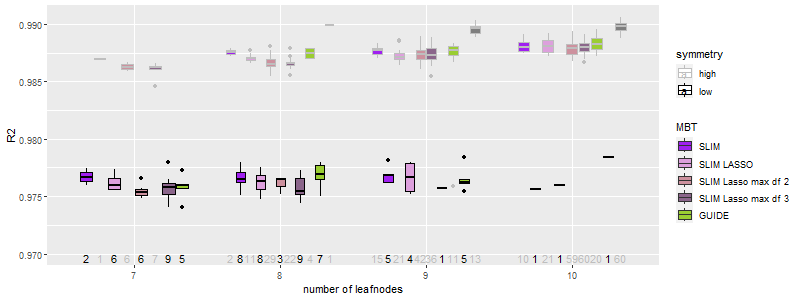
\includegraphics[width=16cm]{Figures/simulations/batchtools/lasso/lasso_standalone_r2_test_slim.png}
    \label{fig:app_lasso_standalone_r2_test_slim}
\end{figure} 

\subsubsection{Nonlinear mixed}



\clearpage
\subsection{Insurance use case}
\subsubsection{K2204 BPV}

 \begin{figure}[!htb]
     \centering     
     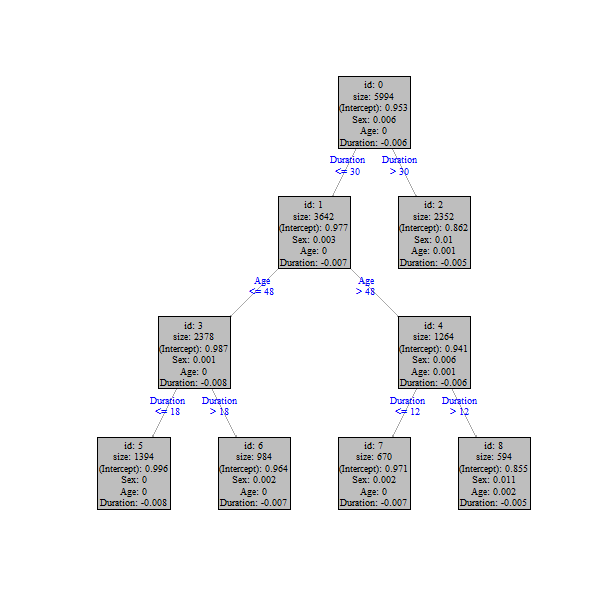
\includegraphics[width = 14cm]{Figures/insurance_use_case/k2204_BPV/slim_lm_tree.png}
     \caption{SLIM tree with linear models as standalone model for BPV in data set K2204}
     \label{fig:app_ins_slim_lm_standalone_tree}
 \end{figure}




\subsubsection{K2204 PPV}
All plots and tables shown in the chapter \ref{K2204_BPV} for the data set k2204 with target BPV are shown here for the target PPV (or PPV\_pred). The interpretation can be done analogously to chapter \ref{K2204_BPV}. The effects found here are merely all larger (since PPV is also larger than BPV) and their direction is exactly reversed. 

\begin{table}[!htb]
\caption{Fidelity of K2204 PPV linear baseline model and linear MBTs}
\centering \scriptsize
\begin{tabular}[t]{l|r|r|r|r|r}
\hline
  & $R^2$ & MSE & MAE & max AE & n leaves\\
\hline
linear baseline model & 0.985092 & 2.523500 & 1.277544 & 7.271319 & 1\\
\hline
SLIM & 0.999232 & 0.130069 & 0.255018 & 2.300768 & 8\\
GUIDE & 0.999275 & 0.122765 & 0.240393 & 2.300768 & 8\\
MOB & 0.998524 & 0.249776 & 0.353372 & 2.758192 & 8\\
CTree & 0.995088 & 0.831537 & 0.643819 & 4.808448 & 8\\
\hline
\end{tabular}
\label{tab:ins_k2204_ppv_lm_surrogates_perf}
\end{table}


\begin{table}[!htb]
\caption{Share of observations split by the different features K2204 PPV linear MBTs}
\centering \scriptsize
\begin{tabular}[t]{l|r|r|r}
\hline
& age & duration & sex\\
\hline
SLIM & 0.28 & 0.67 & 0.05\\
GUIDE & 0.28 & 0.72 & 0.00\\
MOB & 0.10 & 0.77 & 0.13\\
CTree & 0.00 & 0.96 & 0.04\\
\hline
\end{tabular}
\label{tab:ins_k2204_ppv_lm_surrogates_share}
\end{table}



Figure \ref{fig:ins_k2204_ppv_fit} plots the prediction of the baseline B-spline model and the two B-spline SLIM surrogates against PPV\_pred to visualise performance improvement. 

\begin{figure}[!htb]
    \centering    
    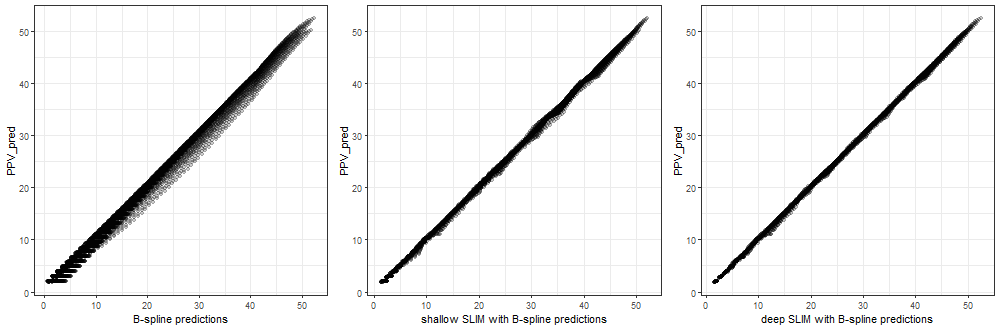
\includegraphics[width = 14cm]{Figures/insurance_use_case/k2204_PPV/fit.png}
    \caption{B-spline surrogate predictions vs. PPV\_pred for K2204}
    \label{fig:ins_k2204_ppv_fit}
\end{figure}

The fidelity results for all B-spline surrogates are listed in table \ref{tab:ins_k2204_ppv_bsplines_surrogates_perf} .

\begin{table}

\caption{Fidelity of K2204 PPV B-spline baseline model and  B-spline MBTs}
\centering \scriptsize
\begin{tabular}[t]{l|r|r|r|r|r}
\hline
  & $R^2$ & MSE & MAE & max AE & n leaves\\
\hline
B-spline baseline model & 0.9943260 & 0.9604583 & 0.7605289 & 4.249894 & 1\\
\hline
SLIM shallow & 0.9994172 & 0.0986492 & 0.2046541 & 1.880490 & 8\\
GUIDE shallow & 0.9993896 & 0.1033306 & 0.2132615 & 1.849715 & 8\\
MOB shallow & 0.9992104 & 0.1336634 & 0.2494695 & 2.063691 & 8\\
CTree shallow & 0.9990906 & 0.1539409 & 0.2713325 & 2.069590 & 8\\
\hline
SLIM deep & 0.9997505 & 0.0422310 & 0.1208647 & 1.421309 & 21\\
GUIDE deep & 0.9997299 & 0.0457276 & 0.1315567 & 1.307047 & 20\\
MOB deep & 0.9996846 & 0.0533855 & 0.1510094 & 1.342777 & 21\\
CTree deep & 0.9997083 & 0.0493729 & 0.1451053 & 1.385141 & 20\\
\hline
\end{tabular}
\label{tab:ins_k2204_ppv_bsplines_surrogates_perf}
\end{table}





Table \ref{tab:ins_k2204_ppv_bsplines_surrogates_share}  shows the proportions of observations that were split according to the different features. 


\begin{table}[!htb]
\caption{Share of observations split by the different features K2204 PPV B-spline MBTs}
\centering \scriptsize
\begin{tabular}[t]{l|r|r|r}
\hline
  & age & duration & sex\\
\hline
SLIM shallow & 0.38 & 0.62 & 0.00\\
GUIDE shallow & 0.30 & 0.70 & 0.00\\
MOB shallow & 0.08 & 0.84 & 0.08\\
CTree shallow & 0.23 & 0.71 & 0.07\\
\hline
SLIM deep & 0.35 & 0.60 & 0.04\\
GUIDE deep & 0.20 & 0.78 & 0.02\\
MOB deep & 0.08 & 0.76 & 0.16\\
CTree deep & 0.20 & 0.67 & 0.13\\
\hline
\end{tabular}
\label{tab:ins_k2204_ppv_bsplines_surrogates_share}
\end{table}



\begin{figure}[!htb]
    \centering   
    \includegraphics[width = 16cm]{Figures/insurance_use_case/k2204_PPV/slim_bsplines_small_tree.png}
         \caption{SLIM tree for K2204 PPV with B-spline models}
     \label{fig:ins_k2204_ppv_slim_bsplines_tree}
\end{figure}



\begin{figure}[!htb]
    \centering
    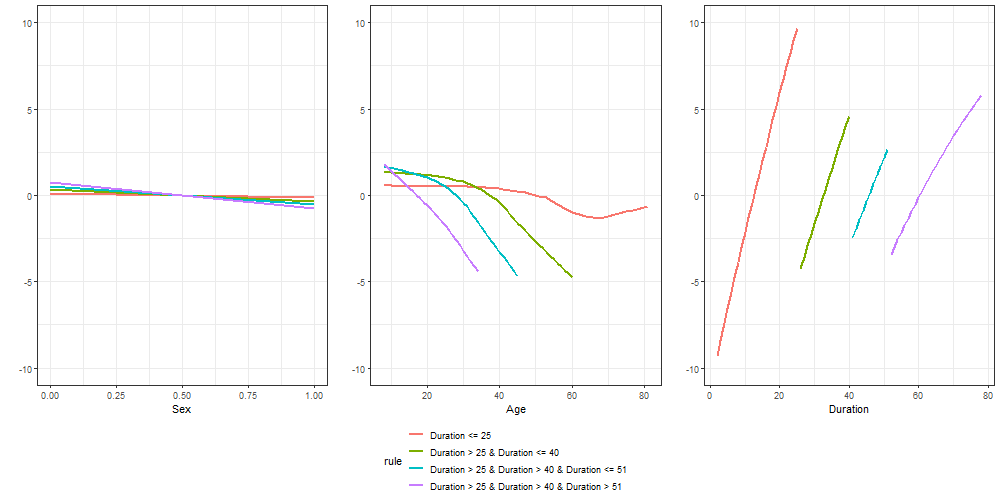
\includegraphics[width = 16cm]{Figures/insurance_use_case/k2204_PPV/effects_duration.png}
    \caption{Input-output relation of features in nodes split by duration for SLIM tree with B-splines and depth 3}
    \label{fig:ins_k2204_ppv_effects_duration}
\end{figure}




\begin{figure}[!htb]
    \centering    
    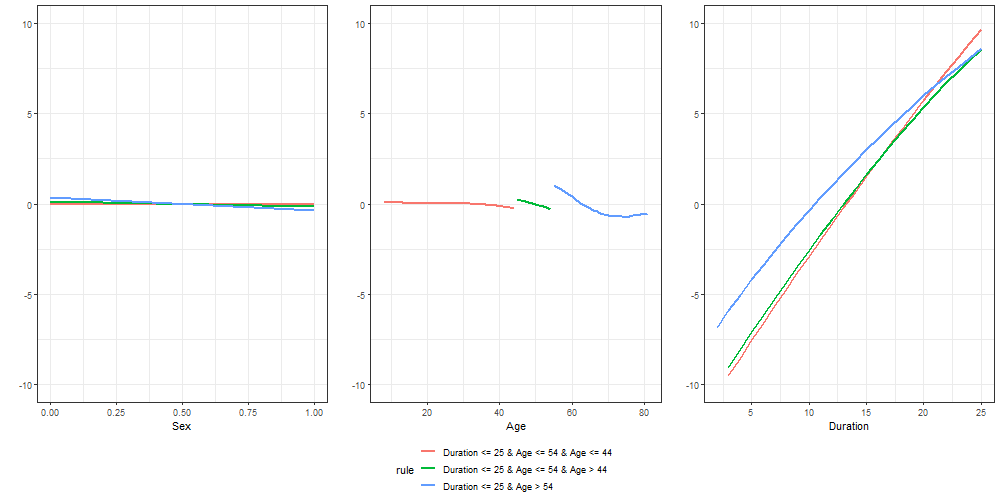
\includegraphics[width = 16cm]{Figures/insurance_use_case/k2204_PPV/effects_age_low_duration.png}
    \caption{Input-output relation of features in nodes with duration $\leq 25$ split by age for SLIM tree with B-splines and depth 3}
    \label{fig:ins_k2204_ppv_effects_age_low_duration}
\end{figure}

\begin{figure}[!htb]
    \centering    
    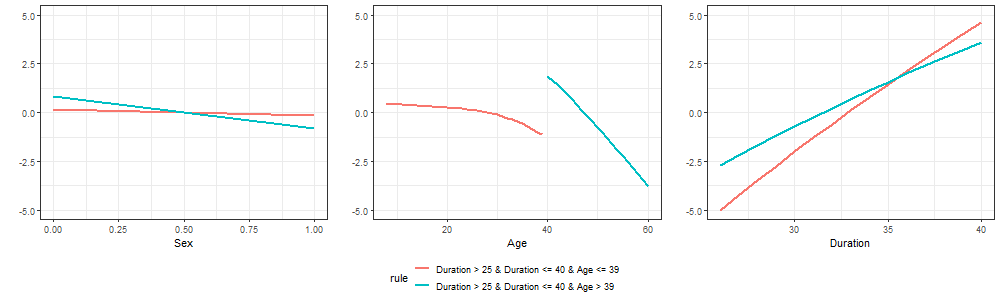
\includegraphics[width = 16cm]{Figures/insurance_use_case/k2204_PPV/effects_age_medium_duration.png}
    \caption{Input-output relation of features in nodes with $25 > $duration $<= 40$ split by age for SLIM tree with B-splines and depth 3}
    \label{fig:ins_k2204_ppv_effects_age_medium_duration}
\end{figure}


\begin{table}[!htb]

\caption{Accuracy of standalone B-spline SLIM MBTs and of the black box model K2204 PPV}
\centering \scriptsize
\begin{tabular}[t]{l|r|r|r|r}
\hline
  & $R^2$ & MSE & MAE & max AE \\
\hline
SLIM & 0.9997757 & 0.0383432 & 0.1140380 & 1.3335727\\
Blackbox model & 0.9998305 & 0.0289638 & 0.1060365 & 0.5345493\\
\hline
\end{tabular}
\label{tab:ins_k2204_ppv_standalone_slim}
\end{table}








\newpage
\clearpage

\section{Electronic appendix}
\label{el_app}

Data, code and figures are provided in electronic form at \url{https://github.com/slds-lmu/msc_2022_loibl_thesis}.
All simulations and evaluations were carried out using the statistical software $\mathtt{R}$ \citep{RCoreTeam.2022}.
The simulations were carried out on the Linux cluster of the Leibniz Supercomputing Centre using the package $\mathtt{batchtools}$ \citep{Lang.2017}.
The author gratefully acknowledge the Leibniz Supercomputing Centre for funding this project by providing computing time on its Linux-Cluster.
For data manipulation, the packages $\mathtt{data.table}$ \citep{Dowle.2021}, $\mathtt{dplyr}$ \citep{Wickham.2022} and $\mathtt{stringr}$ \citep{Wickham.2022b} were used. Visualization was done with $\mathtt{ggplot2}$ \citep{Wickham.2016}, $\mathtt{GGally}$ \citep{Schloerke.2021}, $\mathtt{ggpubr}$ \citep{Kassambara.2020} and $\mathtt{igraph}$ \citep{Csardi.2006}. For fitting the black box xgboost models, the package $\mathtt{mlr3}$ \citep{Lang.2019} was used.

\newpage
\clearpage
    


% ------------------------------------------------------------------------------
% DECLARATION OF AUTHORSHIP-----------------------------------------------------
% ------------------------------------------------------------------------------

\Large
\noindent
\textbf{Declaration of authorship} 
\vspace{0.5cm}
\noindent
\normalsize

I hereby declare that the report submitted is my own unaided work. All direct 
or indirect sources used are acknowledged as references. I am aware that the 
Thesis in digital form can be examined for the use of unauthorized aid and in 
order to determine whether the report as a whole or parts incorporated in it may 
be deemed as plagiarism. For the comparison of my work with existing sources I 
agree that it shall be entered in a database where it shall also remain after 
examination, to enable comparison with future Theses submitted. Further rights 
of reproduction and usage, however, are not granted here. This paper was not 
previously presented to another examination board and has not been published.
\\

\vspace{1cm}
\textcolor{orange}{Location, date} \\

\vspace{3cm}

\noindent\rule{0.5\textwidth}{0.4pt} \\

\textcolor{orange}{Name}

% ------------------------------------------------------------------------------

\end{document}
